\PassOptionsToPackage{unicode=true}{hyperref} % options for packages loaded elsewhere
\PassOptionsToPackage{hyphens}{url}
%
\documentclass[
]{article}
\usepackage{lmodern}
\usepackage{amssymb,amsmath}
\usepackage{ifxetex,ifluatex}
\ifnum 0\ifxetex 1\fi\ifluatex 1\fi=0 % if pdftex
  \usepackage[T1]{fontenc}
  \usepackage[utf8]{inputenc}
  \usepackage{textcomp} % provides euro and other symbols
\else % if luatex or xelatex
  \usepackage{unicode-math}
  \defaultfontfeatures{Scale=MatchLowercase}
  \defaultfontfeatures[\rmfamily]{Ligatures=TeX,Scale=1}
\fi
% use upquote if available, for straight quotes in verbatim environments
\IfFileExists{upquote.sty}{\usepackage{upquote}}{}
\IfFileExists{microtype.sty}{% use microtype if available
  \usepackage[]{microtype}
  \UseMicrotypeSet[protrusion]{basicmath} % disable protrusion for tt fonts
}{}
\makeatletter
\@ifundefined{KOMAClassName}{% if non-KOMA class
  \IfFileExists{parskip.sty}{%
    \usepackage{parskip}
  }{% else
    \setlength{\parindent}{0pt}
    \setlength{\parskip}{6pt plus 2pt minus 1pt}}
}{% if KOMA class
  \KOMAoptions{parskip=half}}
\makeatother
\usepackage{xcolor}
\IfFileExists{xurl.sty}{\usepackage{xurl}}{} % add URL line breaks if available
\IfFileExists{bookmark.sty}{\usepackage{bookmark}}{\usepackage{hyperref}}
\hypersetup{
  pdftitle={ReadMe1},
  pdfauthor={ld},
  pdfborder={0 0 0},
  breaklinks=true}
\urlstyle{same}  % don't use monospace font for urls
\usepackage[margin=1in]{geometry}
\usepackage{color}
\usepackage{fancyvrb}
\newcommand{\VerbBar}{|}
\newcommand{\VERB}{\Verb[commandchars=\\\{\}]}
\DefineVerbatimEnvironment{Highlighting}{Verbatim}{commandchars=\\\{\}}
% Add ',fontsize=\small' for more characters per line
\usepackage{framed}
\definecolor{shadecolor}{RGB}{248,248,248}
\newenvironment{Shaded}{\begin{snugshade}}{\end{snugshade}}
\newcommand{\AlertTok}[1]{\textcolor[rgb]{0.94,0.16,0.16}{#1}}
\newcommand{\AnnotationTok}[1]{\textcolor[rgb]{0.56,0.35,0.01}{\textbf{\textit{#1}}}}
\newcommand{\AttributeTok}[1]{\textcolor[rgb]{0.77,0.63,0.00}{#1}}
\newcommand{\BaseNTok}[1]{\textcolor[rgb]{0.00,0.00,0.81}{#1}}
\newcommand{\BuiltInTok}[1]{#1}
\newcommand{\CharTok}[1]{\textcolor[rgb]{0.31,0.60,0.02}{#1}}
\newcommand{\CommentTok}[1]{\textcolor[rgb]{0.56,0.35,0.01}{\textit{#1}}}
\newcommand{\CommentVarTok}[1]{\textcolor[rgb]{0.56,0.35,0.01}{\textbf{\textit{#1}}}}
\newcommand{\ConstantTok}[1]{\textcolor[rgb]{0.00,0.00,0.00}{#1}}
\newcommand{\ControlFlowTok}[1]{\textcolor[rgb]{0.13,0.29,0.53}{\textbf{#1}}}
\newcommand{\DataTypeTok}[1]{\textcolor[rgb]{0.13,0.29,0.53}{#1}}
\newcommand{\DecValTok}[1]{\textcolor[rgb]{0.00,0.00,0.81}{#1}}
\newcommand{\DocumentationTok}[1]{\textcolor[rgb]{0.56,0.35,0.01}{\textbf{\textit{#1}}}}
\newcommand{\ErrorTok}[1]{\textcolor[rgb]{0.64,0.00,0.00}{\textbf{#1}}}
\newcommand{\ExtensionTok}[1]{#1}
\newcommand{\FloatTok}[1]{\textcolor[rgb]{0.00,0.00,0.81}{#1}}
\newcommand{\FunctionTok}[1]{\textcolor[rgb]{0.00,0.00,0.00}{#1}}
\newcommand{\ImportTok}[1]{#1}
\newcommand{\InformationTok}[1]{\textcolor[rgb]{0.56,0.35,0.01}{\textbf{\textit{#1}}}}
\newcommand{\KeywordTok}[1]{\textcolor[rgb]{0.13,0.29,0.53}{\textbf{#1}}}
\newcommand{\NormalTok}[1]{#1}
\newcommand{\OperatorTok}[1]{\textcolor[rgb]{0.81,0.36,0.00}{\textbf{#1}}}
\newcommand{\OtherTok}[1]{\textcolor[rgb]{0.56,0.35,0.01}{#1}}
\newcommand{\PreprocessorTok}[1]{\textcolor[rgb]{0.56,0.35,0.01}{\textit{#1}}}
\newcommand{\RegionMarkerTok}[1]{#1}
\newcommand{\SpecialCharTok}[1]{\textcolor[rgb]{0.00,0.00,0.00}{#1}}
\newcommand{\SpecialStringTok}[1]{\textcolor[rgb]{0.31,0.60,0.02}{#1}}
\newcommand{\StringTok}[1]{\textcolor[rgb]{0.31,0.60,0.02}{#1}}
\newcommand{\VariableTok}[1]{\textcolor[rgb]{0.00,0.00,0.00}{#1}}
\newcommand{\VerbatimStringTok}[1]{\textcolor[rgb]{0.31,0.60,0.02}{#1}}
\newcommand{\WarningTok}[1]{\textcolor[rgb]{0.56,0.35,0.01}{\textbf{\textit{#1}}}}
\usepackage{graphicx,grffile}
\makeatletter
\def\maxwidth{\ifdim\Gin@nat@width>\linewidth\linewidth\else\Gin@nat@width\fi}
\def\maxheight{\ifdim\Gin@nat@height>\textheight\textheight\else\Gin@nat@height\fi}
\makeatother
% Scale images if necessary, so that they will not overflow the page
% margins by default, and it is still possible to overwrite the defaults
% using explicit options in \includegraphics[width, height, ...]{}
\setkeys{Gin}{width=\maxwidth,height=\maxheight,keepaspectratio}
\setlength{\emergencystretch}{3em}  % prevent overfull lines
\providecommand{\tightlist}{%
  \setlength{\itemsep}{0pt}\setlength{\parskip}{0pt}}
\setcounter{secnumdepth}{-2}
% Redefines (sub)paragraphs to behave more like sections
\ifx\paragraph\undefined\else
  \let\oldparagraph\paragraph
  \renewcommand{\paragraph}[1]{\oldparagraph{#1}\mbox{}}
\fi
\ifx\subparagraph\undefined\else
  \let\oldsubparagraph\subparagraph
  \renewcommand{\subparagraph}[1]{\oldsubparagraph{#1}\mbox{}}
\fi

% set default figure placement to htbp
\makeatletter
\def\fps@figure{htbp}
\makeatother


\title{ReadMe1}
\author{ld}
\date{2021/4/14}

\begin{document}
\maketitle

The goal of crosslink is to visualize the network of grouped nodes

\hypertarget{installation}{%
\subsection{1. Installation}\label{installation}}

You can install the released version of crosslink from
\href{https://github.com/zzwch/crosslink}{github} with:

\begin{Shaded}
\begin{Highlighting}[]
\NormalTok{devtools}\OperatorTok{::}\KeywordTok{install_github}\NormalTok{(}\StringTok{"zzwch/crosslinks"}\NormalTok{) }
\end{Highlighting}
\end{Shaded}

\begin{verbatim}
## Skipping install of 'crosslinks' from a github remote, the SHA1 (0669475c) has not changed since last install.
##   Use `force = TRUE` to force installation
\end{verbatim}

\begin{Shaded}
\begin{Highlighting}[]
\KeywordTok{library}\NormalTok{(crosslink)}
\end{Highlighting}
\end{Shaded}

\begin{verbatim}
## Loading required package: ggplot2
\end{verbatim}

\begin{verbatim}
## Loading required package: magrittr
\end{verbatim}

\hypertarget{quick-start}{%
\subsection{2. Quick start}\label{quick-start}}

Examples of typical crosslonk usage.

\begin{Shaded}
\begin{Highlighting}[]
\NormalTok{cl <-}\StringTok{ }\KeywordTok{crosslink}\NormalTok{(demo}\OperatorTok{$}\NormalTok{nodes, demo}\OperatorTok{$}\NormalTok{edges, demo}\OperatorTok{$}\NormalTok{cross.by, }\DataTypeTok{odd.rm =}\NormalTok{ F,}\DataTypeTok{spaces =} \StringTok{"flank"}\NormalTok{)}
\NormalTok{cl }\OperatorTok\StringTok{ }\KeywordTok{cl_plot}\NormalTok{()}
\end{Highlighting}
\end{Shaded}

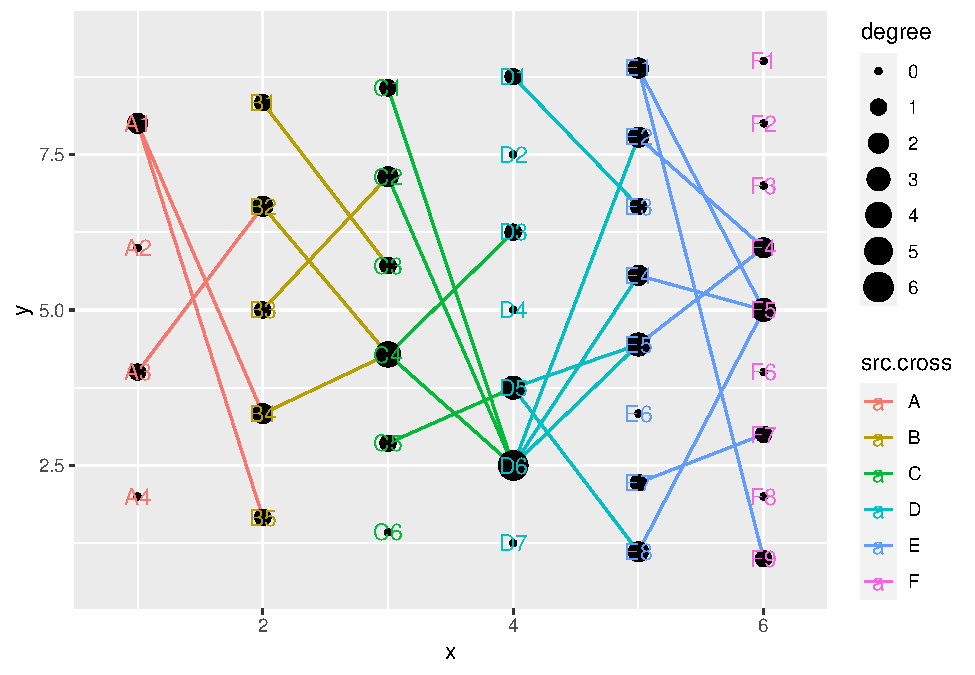
\includegraphics{ReadMe1_files/figure-latex/unnamed-chunk-3-1.pdf}

\hypertarget{step-by-step}{%
\subsection{3. Step by step}\label{step-by-step}}

This is a basic example of the basic function of crosslink
packages,including 1). Input data 2). Generate CrossLink class 3).
Coordinate transformation 4). Layout modules 5). Plotting modules

\hypertarget{input-data}{%
\subsubsection{1). Input data}\label{input-data}}

crosslink needs two files as input. a. nodes (must have two columns:
node name and node type) b. edges data (must have two columns: source
node and target node).

crosslink also provides the function `gen\_demo' to generate demo data.

\begin{Shaded}
\begin{Highlighting}[]
\CommentTok{# generate demo data}
\NormalTok{n <-}\StringTok{ }\DecValTok{6}
\NormalTok{demo <-}\StringTok{ }\KeywordTok{gen_demo}\NormalTok{(}\DataTypeTok{n_cross =}\NormalTok{ n,}\DataTypeTok{n_node =} \DecValTok{4}\OperatorTok{:}\NormalTok{(n}\OperatorTok{+}\DecValTok{3}\NormalTok{), }\DataTypeTok{n_link =} \DecValTok{3}\OperatorTok{:}\NormalTok{(n}\OperatorTok{+}\DecValTok{1}\NormalTok{), }\DataTypeTok{seed =} \DecValTok{66}\NormalTok{)}
\NormalTok{nodes <-}\StringTok{ }\NormalTok{demo}\OperatorTok{$}\NormalTok{nodes}
\NormalTok{edges <-}\StringTok{ }\NormalTok{demo}\OperatorTok{$}\NormalTok{edges}
\NormalTok{cross.by <-}\StringTok{ }\NormalTok{demo}\OperatorTok{$}\NormalTok{cross.by}
\end{Highlighting}
\end{Shaded}

\hypertarget{generate-crosslink-class}{%
\subsubsection{2). Generate crossLink
class}\label{generate-crosslink-class}}

crosslink can help to generate an object of crosslink class for plot.

\begin{Shaded}
\begin{Highlighting}[]
\CommentTok{# users can define 'odd.rm' to choose if remove the nodes have zero relationship with any other nodes when generate crosslink class}
\CommentTok{# user can set intervals between nodes and gaps through spaces and gaps.}
\NormalTok{cl <-}\StringTok{ }\KeywordTok{crosslink}\NormalTok{(nodes, edges, cross.by, }\DataTypeTok{odd.rm =}\NormalTok{ F,}\DataTypeTok{spaces =} \StringTok{"flank"}\NormalTok{)}

\NormalTok{cl }\OperatorTok\StringTok{ }\KeywordTok{get_cross}\NormalTok{()   }\CommentTok{# get node information}
\end{Highlighting}
\end{Shaded}

\begin{verbatim}
##     node node.type x        y cross key type degree
## A2    A4      node 1 2.000000     A  A4    A      0
## A3    A3      node 1 4.000000     A  A3    A      1
## A4    A2      node 1 6.000000     A  A2    A      0
## A5    A1      node 1 8.000000     A  A1    A      2
## B2    B5      node 2 1.666667     B  B5    B      1
## B3    B4      node 2 3.333333     B  B4    B      2
## B4    B3      node 2 5.000000     B  B3    B      1
## B5    B2      node 2 6.666667     B  B2    B      2
## B6    B1      node 2 8.333333     B  B1    B      1
## C2    C6      node 3 1.428571     C  C6    C      0
## C3    C5      node 3 2.857143     C  C5    C      1
## C4    C4      node 3 4.285714     C  C4    C      4
## C5    C3      node 3 5.714286     C  C3    C      1
## C6    C2      node 3 7.142857     C  C2    C      2
## C7    C1      node 3 8.571429     C  C1    C      1
## D2    D7      node 4 1.250000     D  D7    D      0
## D3    D6      node 4 2.500000     D  D6    D      6
## D4    D5      node 4 3.750000     D  D5    D      3
## D5    D4      node 4 5.000000     D  D4    D      0
## D6    D3      node 4 6.250000     D  D3    D      1
## D7    D2      node 4 7.500000     D  D2    D      0
## D8    D1      node 4 8.750000     D  D1    D      1
## E2    E8      node 5 1.111111     E  E8    E      2
## E3    E7      node 5 2.222222     E  E7    E      1
## E4    E6      node 5 3.333333     E  E6    E      0
## E5    E5      node 5 4.444444     E  E5    E      3
## E6    E4      node 5 5.555556     E  E4    E      2
## E7    E3      node 5 6.666667     E  E3    E      1
## E8    E2      node 5 7.777778     E  E2    E      2
## E9    E1      node 5 8.888889     E  E1    E      2
## F2    F9      node 6 1.000000     F  F9    F      1
## F3    F8      node 6 2.000000     F  F8    F      0
## F4    F7      node 6 3.000000     F  F7    F      1
## F5    F6      node 6 4.000000     F  F6    F      0
## F6    F5      node 6 5.000000     F  F5    F      3
## F7    F4      node 6 6.000000     F  F4    F      2
## F8    F3      node 6 7.000000     F  F3    F      0
## F9    F2      node 6 8.000000     F  F2    F      0
## F10   F1      node 6 9.000000     F  F1    F      0
\end{verbatim}

\begin{Shaded}
\begin{Highlighting}[]
\NormalTok{cl }\OperatorTok\StringTok{ }\KeywordTok{get_link}\NormalTok{()    }\CommentTok{# get edges information}
\end{Highlighting}
\end{Shaded}

\begin{verbatim}
##    src tar src.cross tar.cross source target x        y xend     yend
## 1   A1  B4         A         B     A1     B4 1 8.000000    2 3.333333
## 2   A3  B2         A         B     A3     B2 1 4.000000    2 6.666667
## 3   A1  B5         A         B     A1     B5 1 8.000000    2 1.666667
## 4   B3  C2         B         C     B3     C2 2 5.000000    3 7.142857
## 5   B2  C4         B         C     B2     C4 2 6.666667    3 4.285714
## 6   B1  C3         B         C     B1     C3 2 8.333333    3 5.714286
## 7   B4  C4         B         C     B4     C4 2 3.333333    3 4.285714
## 8   C4  D3         C         D     C4     D3 3 4.285714    4 6.250000
## 9   C5  D5         C         D     C5     D5 3 2.857143    4 3.750000
## 10  C2  D6         C         D     C2     D6 3 7.142857    4 2.500000
## 11  C4  D6         C         D     C4     D6 3 4.285714    4 2.500000
## 12  C1  D6         C         D     C1     D6 3 8.571429    4 2.500000
## 13  D6  E4         D         E     D6     E4 4 2.500000    5 5.555556
## 14  D6  E5         D         E     D6     E5 4 2.500000    5 4.444444
## 15  D1  E3         D         E     D1     E3 4 8.750000    5 6.666667
## 16  D5  E8         D         E     D5     E8 4 3.750000    5 1.111111
## 17  D6  E2         D         E     D6     E2 4 2.500000    5 7.777778
## 18  D5  E5         D         E     D5     E5 4 3.750000    5 4.444444
## 19  E2  F4         E         F     E2     F4 5 7.777778    6 6.000000
## 20  E4  F5         E         F     E4     F5 5 5.555556    6 5.000000
## 21  E5  F4         E         F     E5     F4 5 4.444444    6 6.000000
## 22  E7  F7         E         F     E7     F7 5 2.222222    6 3.000000
## 23  E8  F5         E         F     E8     F5 5 1.111111    6 5.000000
## 24  E1  F9         E         F     E1     F9 5 8.888889    6 1.000000
## 25  E1  F5         E         F     E1     F5 5 8.888889    6 5.000000
\end{verbatim}

\begin{Shaded}
\begin{Highlighting}[]
\NormalTok{cl }\OperatorTok\StringTok{ }\KeywordTok{cl_layouts}\NormalTok{()  }\CommentTok{# get layouts information of crosslink object}
\end{Highlighting}
\end{Shaded}

\begin{verbatim}
## [1] "default"
\end{verbatim}

\begin{Shaded}
\begin{Highlighting}[]
\NormalTok{cl }\OperatorTok\StringTok{ }\KeywordTok{cl_active}\NormalTok{()   }\CommentTok{# get active layouts information of crosslink object}
\end{Highlighting}
\end{Shaded}

\begin{verbatim}
## [1] "default"
\end{verbatim}

\hypertarget{coordinate-transformation}{%
\subsubsection{3). Coordinate
transformation}\label{coordinate-transformation}}

Coordinate transformation consists of affine transformation and
functional transformation. The \texttt{tf\_affine} function contains
\texttt{tf\_rotate}, \texttt{tf\_shift}, \texttt{tf\_shear},
\texttt{tf\_flip} and \texttt{tf\_scale} function. The \texttt{tf\_fun}
interface allows user to custom transforming function.

\begin{Shaded}
\begin{Highlighting}[]
\CommentTok{# tf_rotate, rotating in a specific angle with (x,y) as the center.}
\NormalTok{cl }\OperatorTok\StringTok{ }\KeywordTok{tf_rotate}\NormalTok{(}\DataTypeTok{x=}\DecValTok{0}\NormalTok{,}\DataTypeTok{y=}\DecValTok{1}\NormalTok{,}\DataTypeTok{angle =} \DecValTok{45}\NormalTok{) }\OperatorTok\StringTok{ }\KeywordTok{cl_plot}\NormalTok{()}
\end{Highlighting}
\end{Shaded}

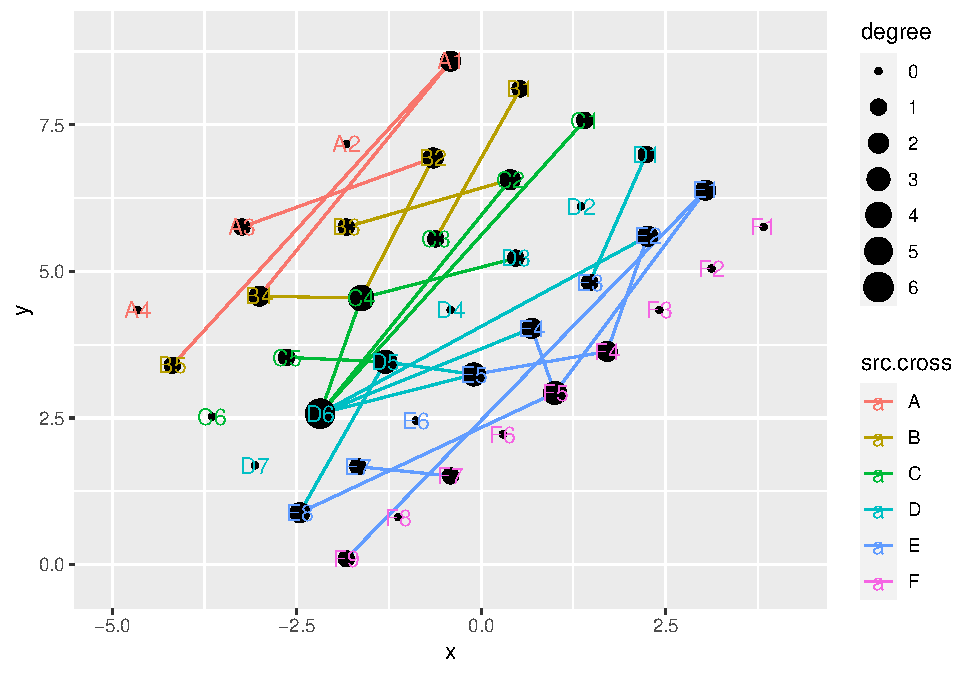
\includegraphics{ReadMe1_files/figure-latex/unnamed-chunk-6-1.pdf}

\begin{Shaded}
\begin{Highlighting}[]
\CommentTok{# tf_shift, shifting a relative distance according to x-axis or y-axis}
\NormalTok{cl }\OperatorTok\StringTok{ }\KeywordTok{tf_shift}\NormalTok{(}\DataTypeTok{x=}\DecValTok{1}\NormalTok{,}\DataTypeTok{y=}\OperatorTok{-}\DecValTok{1}\NormalTok{) }\OperatorTok\StringTok{ }\KeywordTok{cl_plot}\NormalTok{()}
\end{Highlighting}
\end{Shaded}

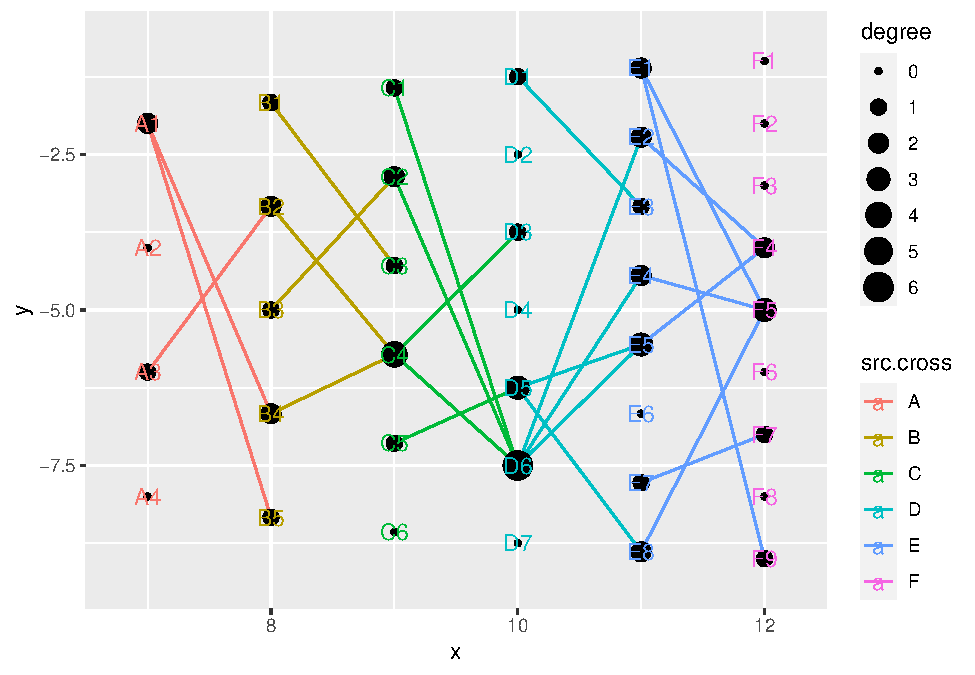
\includegraphics{ReadMe1_files/figure-latex/unnamed-chunk-6-2.pdf}

\begin{Shaded}
\begin{Highlighting}[]
\CommentTok{# tf_shear}
\NormalTok{cl }\OperatorTok\StringTok{ }\KeywordTok{tf_shear}\NormalTok{(}\DataTypeTok{axis =} \StringTok{"x"}\NormalTok{,}\DataTypeTok{angle =} \DecValTok{60}\NormalTok{) }\OperatorTok\StringTok{ }\KeywordTok{cl_plot}\NormalTok{()}
\end{Highlighting}
\end{Shaded}

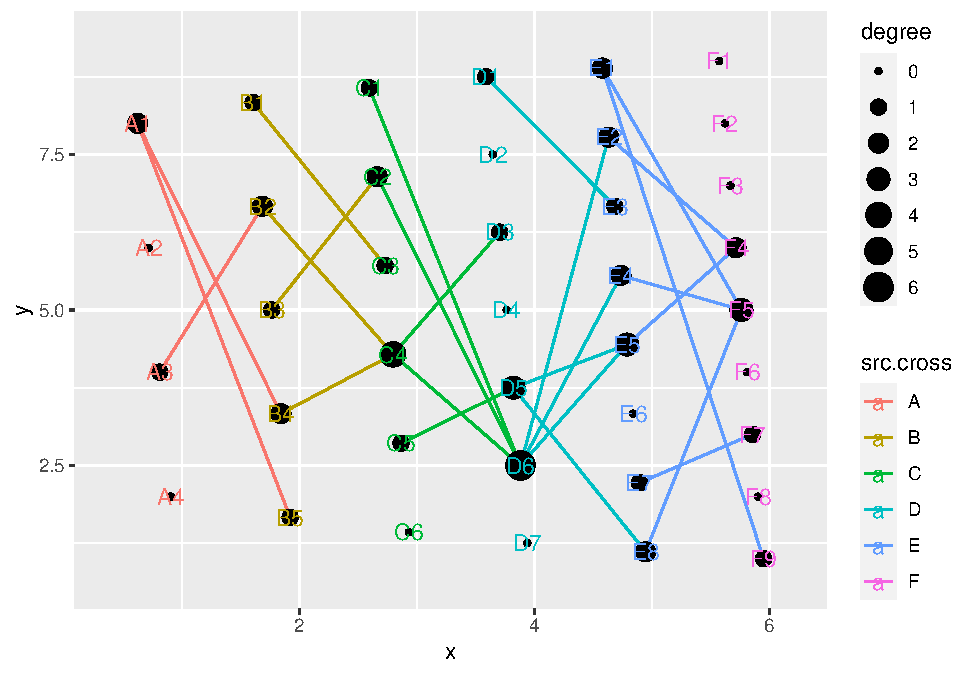
\includegraphics{ReadMe1_files/figure-latex/unnamed-chunk-6-3.pdf}

\begin{Shaded}
\begin{Highlighting}[]
\CommentTok{# tf_flip, flip the figure according to x-axis or y-axis}
\NormalTok{cl }\OperatorTok\StringTok{ }\KeywordTok{tf_flip}\NormalTok{(}\DataTypeTok{axis =} \StringTok{"y"}\NormalTok{) }\OperatorTok\StringTok{ }\KeywordTok{cl_plot}\NormalTok{()}
\end{Highlighting}
\end{Shaded}

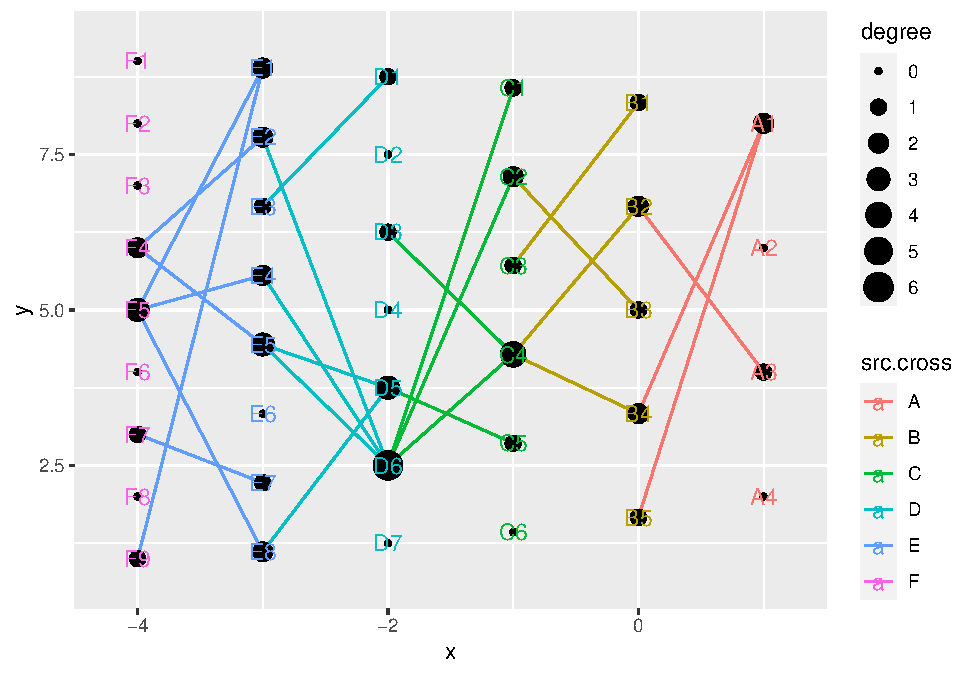
\includegraphics{ReadMe1_files/figure-latex/unnamed-chunk-6-4.pdf}

\begin{Shaded}
\begin{Highlighting}[]
\CommentTok{# tf_scale}
\NormalTok{cl }\OperatorTok\StringTok{ }\KeywordTok{tf_scale}\NormalTok{(}\DataTypeTok{x=}\DecValTok{0}\NormalTok{,}\DataTypeTok{y=}\DecValTok{1}\NormalTok{,}\DataTypeTok{scale =} \DecValTok{5}\NormalTok{) }\OperatorTok\StringTok{ }\KeywordTok{cl_plot}\NormalTok{() }
\end{Highlighting}
\end{Shaded}

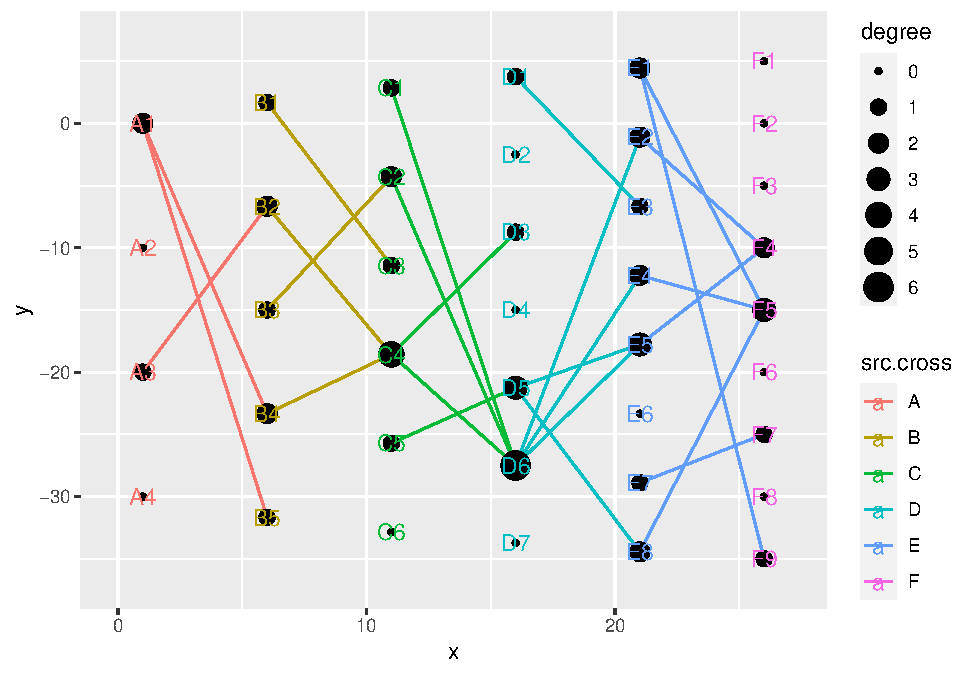
\includegraphics{ReadMe1_files/figure-latex/unnamed-chunk-6-5.pdf}

\begin{Shaded}
\begin{Highlighting}[]
\CommentTok{# tf_fun, coordinate transformation according to custom-defined function}
\NormalTok{cl }\OperatorTok\StringTok{ }\KeywordTok{tf_fun}\NormalTok{(}\DataTypeTok{fun =}\NormalTok{ sin,}\DataTypeTok{along =} \StringTok{"y"}\NormalTok{,}\DataTypeTok{xrange.from=}\KeywordTok{c}\NormalTok{(}\DecValTok{0}\NormalTok{,}\FloatTok{0.5}\OperatorTok{*}\NormalTok{pi)) }\OperatorTok\StringTok{ }\KeywordTok{cl_plot}\NormalTok{()}
\end{Highlighting}
\end{Shaded}

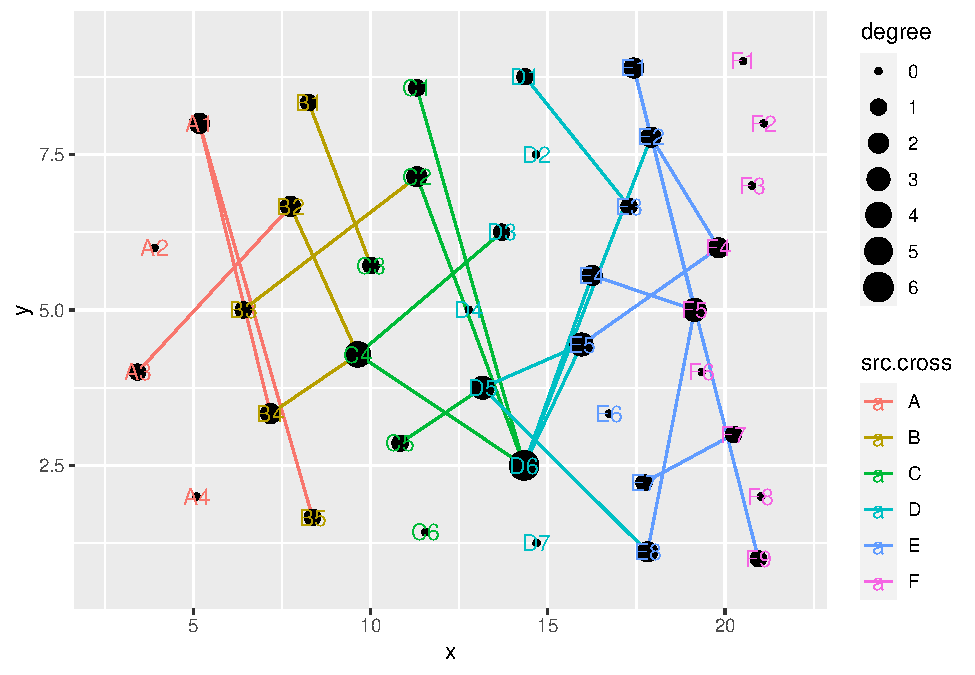
\includegraphics{ReadMe1_files/figure-latex/unnamed-chunk-6-6.pdf}

\begin{Shaded}
\begin{Highlighting}[]
\CommentTok{# combined tf functions}
\NormalTok{cl }\OperatorTok\StringTok{ }\KeywordTok{tf_flip}\NormalTok{(}\DataTypeTok{axis =} \StringTok{"y"}\NormalTok{) }\OperatorTok\StringTok{ }\KeywordTok{tf_fun}\NormalTok{(}\DataTypeTok{fun =}\NormalTok{ sin,}\DataTypeTok{along =} \StringTok{"y"}\NormalTok{,}\DataTypeTok{xrange.from=}\KeywordTok{c}\NormalTok{(}\DecValTok{0}\NormalTok{,}\FloatTok{0.5}\OperatorTok{*}\NormalTok{pi)) }\OperatorTok\StringTok{ }\KeywordTok{cl_plot}\NormalTok{()}
\end{Highlighting}
\end{Shaded}

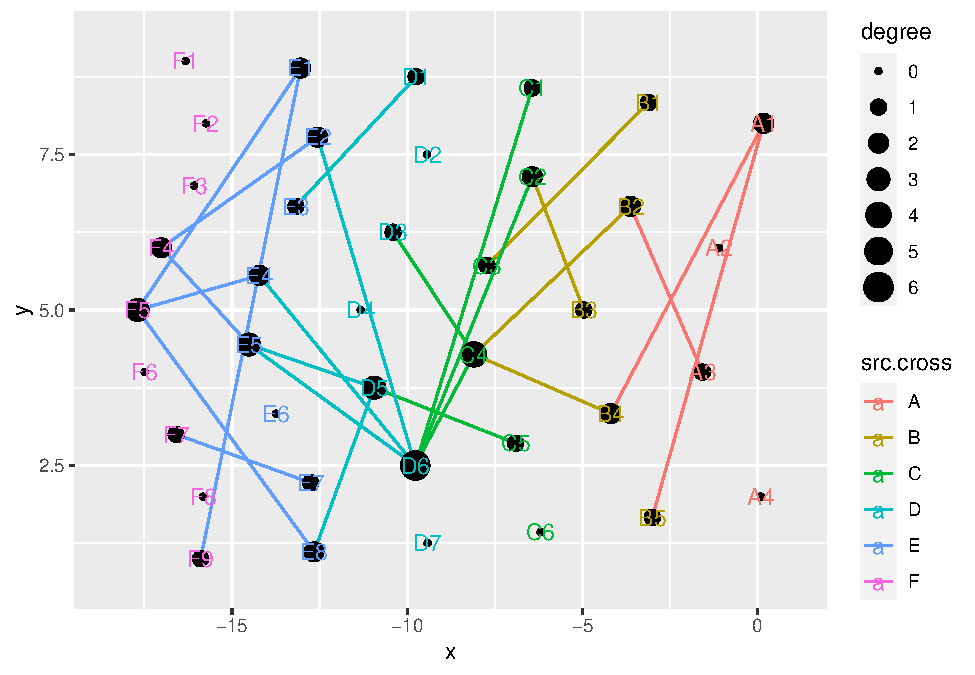
\includegraphics{ReadMe1_files/figure-latex/unnamed-chunk-6-7.pdf}

\hypertarget{layout-modules}{%
\subsubsection{4). Layout modules}\label{layout-modules}}

\begin{enumerate}
\def\labelenumi{\alph{enumi}.}
\tightlist
\item
  Commonly used styles are predefined in layout module, including row,
  column, arc, polygon and hive. crosses can be specified in all five
  layout module
\item
  `set\_header' function is provided to conveniently place cross headers
\end{enumerate}

\begin{Shaded}
\begin{Highlighting}[]
\CommentTok{# default layout module is column}
\NormalTok{cl }\OperatorTok\StringTok{ }\KeywordTok{cl_plot}\NormalTok{()}
\end{Highlighting}
\end{Shaded}

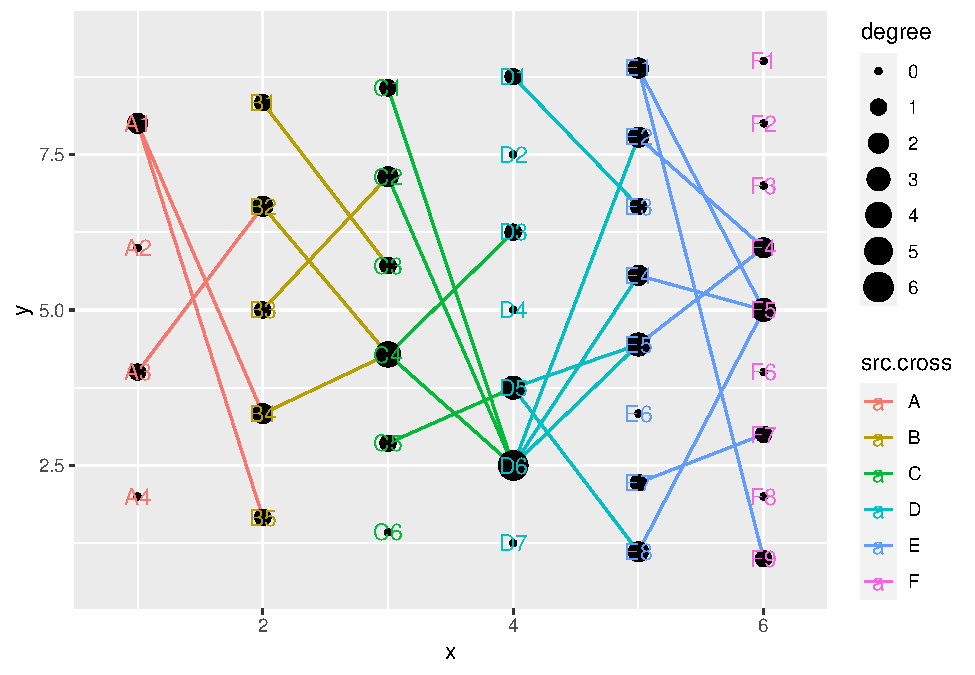
\includegraphics{ReadMe1_files/figure-latex/unnamed-chunk-7-1.pdf}

\begin{Shaded}
\begin{Highlighting}[]
\NormalTok{cl }\OperatorTok\StringTok{ }\KeywordTok{layout_column}\NormalTok{() }\OperatorTok\StringTok{ }\KeywordTok{cl_plot}\NormalTok{()}
\end{Highlighting}
\end{Shaded}

\begin{verbatim}
## Copy layout default into default, and Set active layout to default
## Copy layout default into default, and Set active layout to default
\end{verbatim}

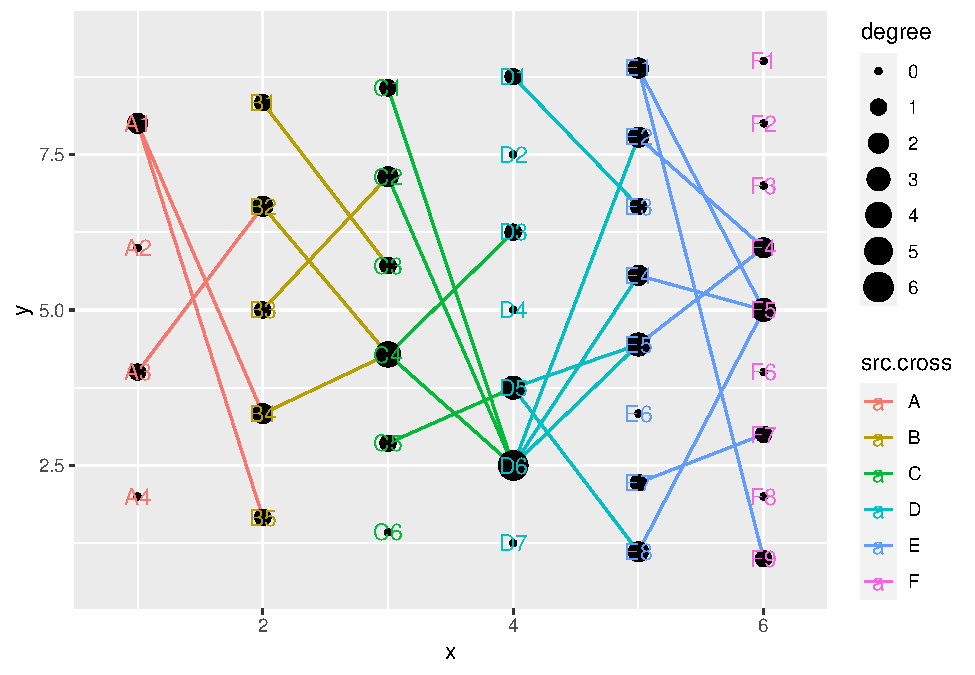
\includegraphics{ReadMe1_files/figure-latex/unnamed-chunk-7-2.pdf}

\begin{Shaded}
\begin{Highlighting}[]
\CommentTok{# layout by row}
\NormalTok{cl }\OperatorTok\StringTok{ }\KeywordTok{layout_row}\NormalTok{() }\OperatorTok\StringTok{ }\KeywordTok{cl_plot}\NormalTok{()}
\end{Highlighting}
\end{Shaded}

\begin{verbatim}
## Copy layout default into default, and Set active layout to default
\end{verbatim}

\begin{verbatim}
## Copy layout temp into default, and Set active layout to default
\end{verbatim}

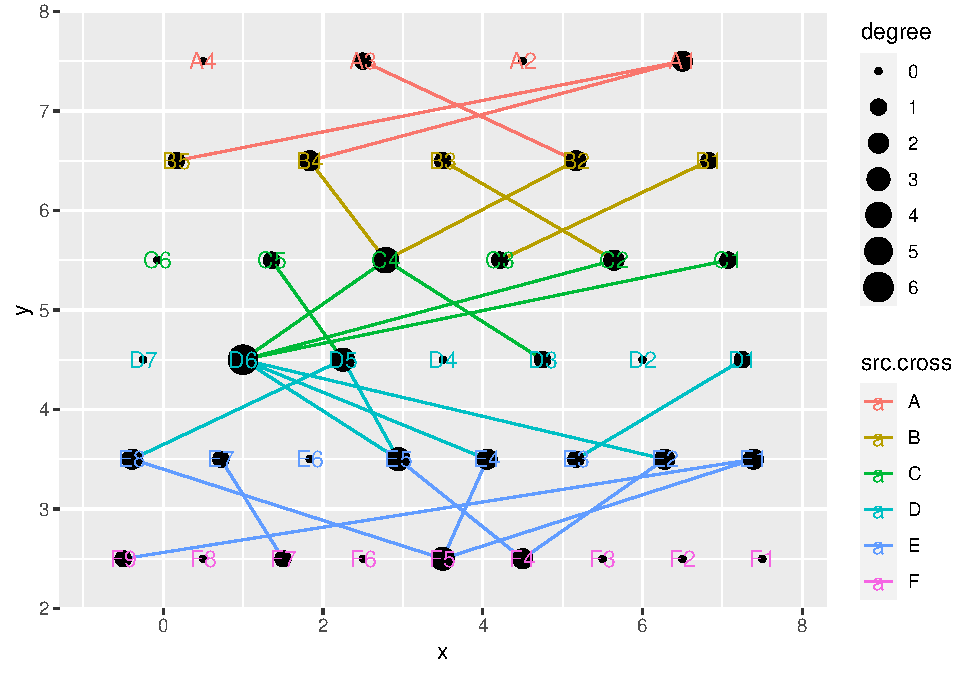
\includegraphics{ReadMe1_files/figure-latex/unnamed-chunk-7-3.pdf}

\begin{Shaded}
\begin{Highlighting}[]
\CommentTok{# layout by arc}
\NormalTok{cl }\OperatorTok\StringTok{ }\KeywordTok{layout_arc}\NormalTok{(}\DataTypeTok{angles =} \DecValTok{60}\NormalTok{,}\DataTypeTok{crosses =} \KeywordTok{c}\NormalTok{(}\StringTok{"E"}\NormalTok{,}\StringTok{"F"}\NormalTok{)) }\OperatorTok\StringTok{ }\KeywordTok{cl_plot}\NormalTok{()}
\end{Highlighting}
\end{Shaded}

\begin{verbatim}
## Copy layout default into temp, and Set active layout to temp
\end{verbatim}

\begin{verbatim}
## Copy layout default into default, and Set active layout to default
\end{verbatim}

\begin{verbatim}
## Copy layout temp into default, and Set active layout to default
\end{verbatim}

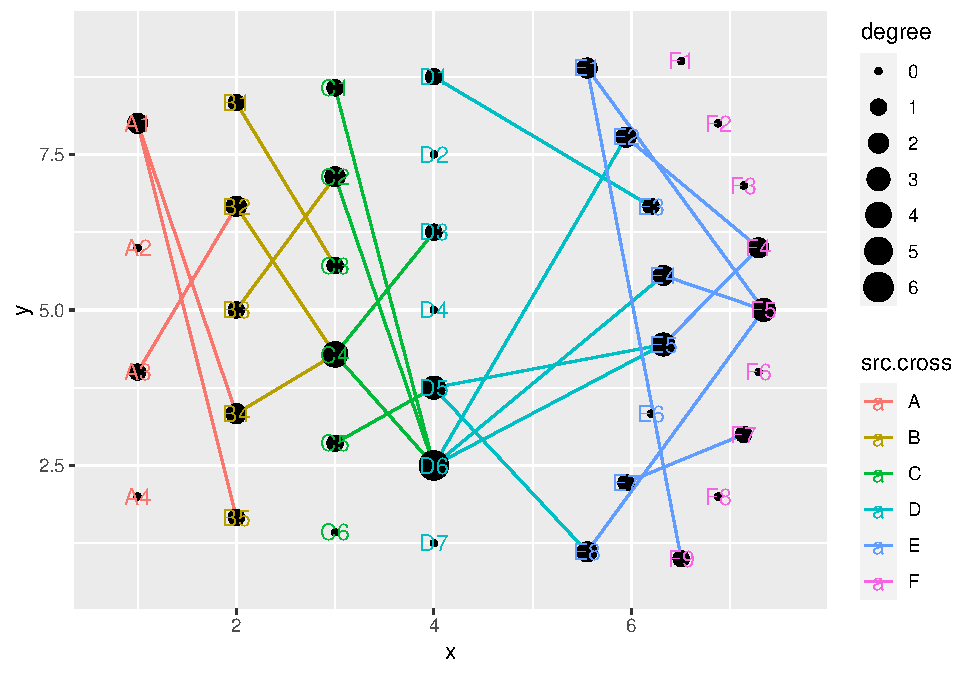
\includegraphics{ReadMe1_files/figure-latex/unnamed-chunk-7-4.pdf}

\begin{Shaded}
\begin{Highlighting}[]
\CommentTok{# layout by polygon (list of angles must have the same length with crosses)}
\NormalTok{cl }\OperatorTok\StringTok{ }\KeywordTok{layout_polygon}\NormalTok{() }\OperatorTok\StringTok{ }\KeywordTok{cl_plot}\NormalTok{()}
\end{Highlighting}
\end{Shaded}

\begin{verbatim}
## Copy layout default into default, and Set active layout to default
## Copy layout temp into default, and Set active layout to default
\end{verbatim}

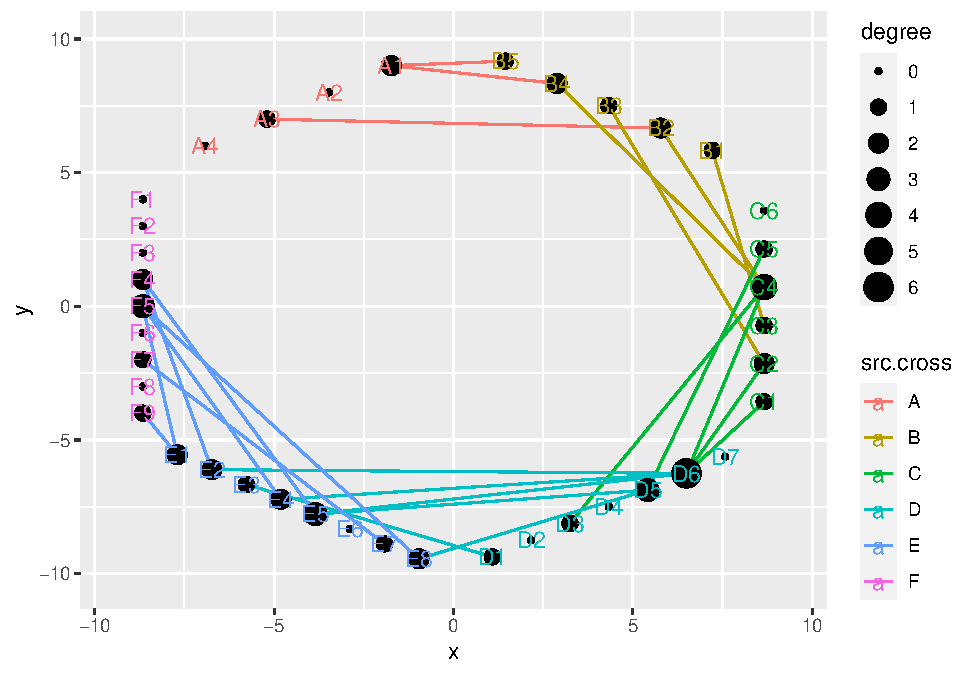
\includegraphics{ReadMe1_files/figure-latex/unnamed-chunk-7-5.pdf}

\begin{Shaded}
\begin{Highlighting}[]
\CommentTok{# layout by hive}
\NormalTok{cl }\OperatorTok\StringTok{ }\KeywordTok{layout_hive}\NormalTok{() }\OperatorTok\StringTok{ }\KeywordTok{cl_plot}\NormalTok{()}
\end{Highlighting}
\end{Shaded}

\begin{verbatim}
## Copy layout default into default, and Set active layout to default
## Copy layout temp into default, and Set active layout to default
\end{verbatim}

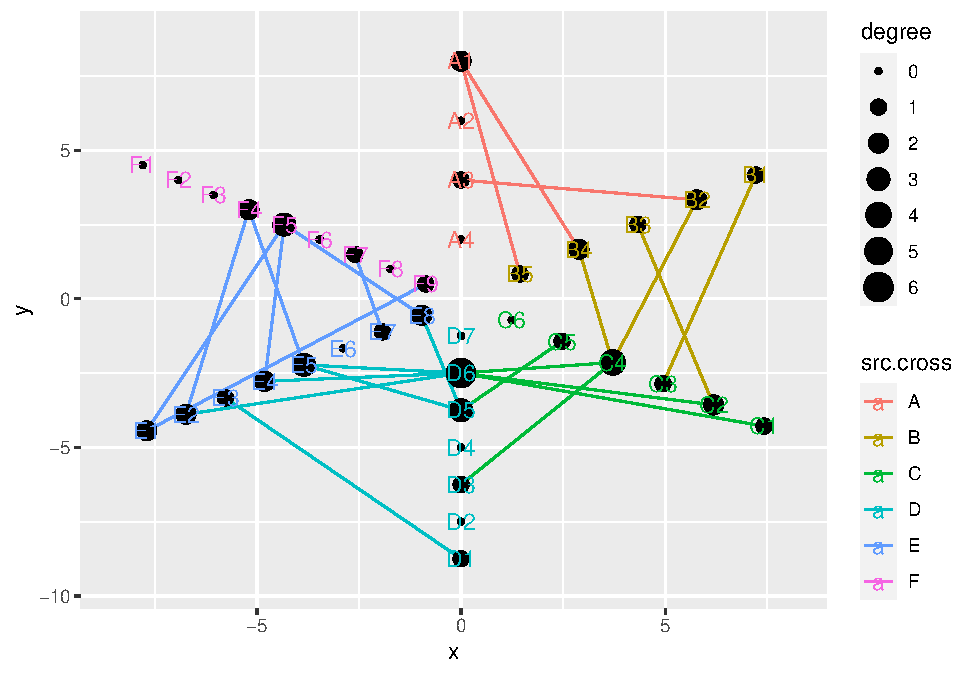
\includegraphics{ReadMe1_files/figure-latex/unnamed-chunk-7-6.pdf}

\begin{Shaded}
\begin{Highlighting}[]
\CommentTok{# Header can be customized through 'set_header'}
\KeywordTok{set_header}\NormalTok{(cl,}\DataTypeTok{header =} \KeywordTok{c}\NormalTok{(}\StringTok{"A"}\NormalTok{,}\StringTok{"B"}\NormalTok{,}\StringTok{"C"}\NormalTok{,}\StringTok{"D"}\NormalTok{,}\StringTok{"E"}\NormalTok{,}\StringTok{"F"}\NormalTok{)) ->}\StringTok{ }\NormalTok{cl}
\NormalTok{cl }\OperatorTok\StringTok{ }\KeywordTok{get_header}\NormalTok{()  }\CommentTok{# get header of crosslink object }
\end{Highlighting}
\end{Shaded}

\begin{verbatim}
##       node node.type x   y cross header
## 1 A_HEADER    header 1 9.5     A      A
## 2 B_HEADER    header 2 9.5     B      B
## 3 C_HEADER    header 3 9.5     C      C
## 4 D_HEADER    header 4 9.5     D      D
## 5 E_HEADER    header 5 9.5     E      E
## 6 F_HEADER    header 6 9.5     F      F
\end{verbatim}

\hypertarget{plotting-modules}{%
\subsubsection{5). Plotting modules}\label{plotting-modules}}

We introduce this pattern in three aspects.

\begin{enumerate}
\def\labelenumi{\alph{enumi}.}
\tightlist
\item
  quick plotting (\texttt{cl\_plot})
\item
  aesthetic settings ( The color, size, type and text of the nodes and
  lines in the network)
\item
  combination of the network diagram with the corresponding node
  annotation image in aligning coordinates
\end{enumerate}

\hypertarget{a.-quick-plotting}{%
\paragraph{a. quick plotting}\label{a.-quick-plotting}}

\begin{Shaded}
\begin{Highlighting}[]
\NormalTok{cl }\OperatorTok\StringTok{ }\KeywordTok{cl_plot}\NormalTok{()}
\end{Highlighting}
\end{Shaded}

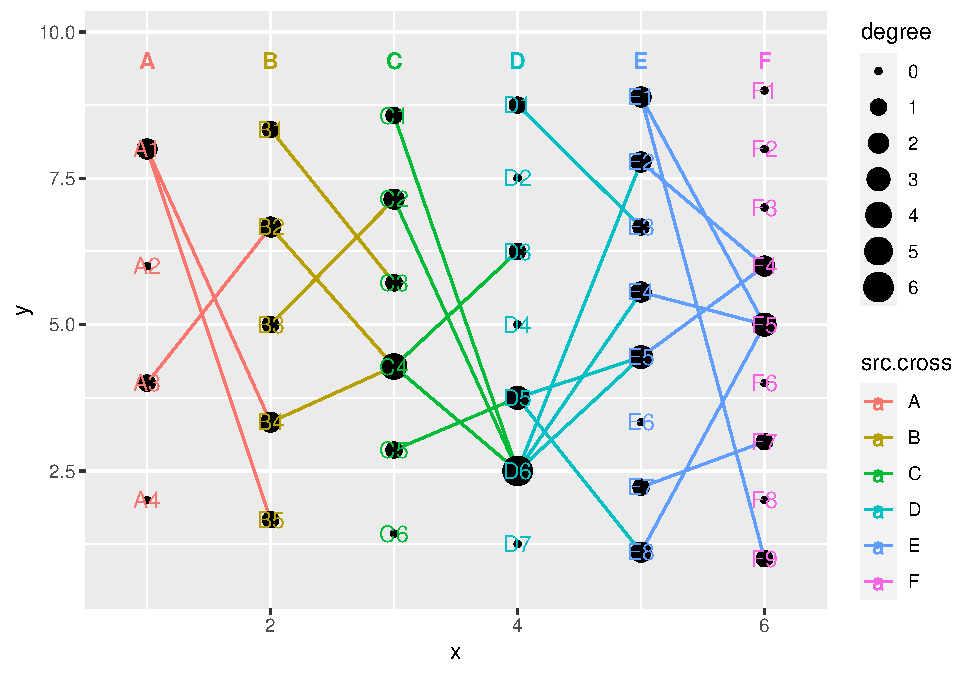
\includegraphics{ReadMe1_files/figure-latex/unnamed-chunk-8-1.pdf}

\hypertarget{b.-aesthetic-settings}{%
\paragraph{b. aesthetic settings}\label{b.-aesthetic-settings}}

\begin{Shaded}
\begin{Highlighting}[]
\CommentTok{# aesthetic settings based on ggplot2 system, some specific examples are shown below.}

\CommentTok{# set colors, shapes and size of nodes}
\CommentTok{# cross:a named list of arguments for crosses. usage same as ggplot2::geom_point(). Set NULL to use default settings, or Set NA to not show.}
\NormalTok{cl }\OperatorTok\StringTok{ }\KeywordTok{cl_plot}\NormalTok{(}\DataTypeTok{cross =} \KeywordTok{list}\NormalTok{(}\DataTypeTok{mapping =}  \KeywordTok{aes}\NormalTok{(}\DataTypeTok{color =}\NormalTok{ type,}\DataTypeTok{shape=}\NormalTok{ type,}\DataTypeTok{size=}\NormalTok{type),}
                            \DataTypeTok{scale   =} \KeywordTok{list}\NormalTok{(}\DataTypeTok{color =} \KeywordTok{scale_color_manual}\NormalTok{(}\DataTypeTok{values =}\NormalTok{ RColorBrewer}\OperatorTok{::}\KeywordTok{brewer.pal}\NormalTok{(}\DecValTok{8}\NormalTok{, }\StringTok{"Set1"}\NormalTok{)),}
                                           \DataTypeTok{size  =} \KeywordTok{scale_size_manual}\NormalTok{(}\DataTypeTok{values =} \KeywordTok{seq}\NormalTok{(}\DecValTok{1}\NormalTok{,}\DecValTok{12}\NormalTok{,}\DataTypeTok{by=}\DecValTok{2}\NormalTok{)),}
                                           \DataTypeTok{shape  =} \KeywordTok{scale_shape_manual}\NormalTok{(}\DataTypeTok{values =} \KeywordTok{c}\NormalTok{(}\DecValTok{15}\OperatorTok{:}\DecValTok{22}\NormalTok{))}
\NormalTok{                                          )}
\NormalTok{                           ))}
\end{Highlighting}
\end{Shaded}

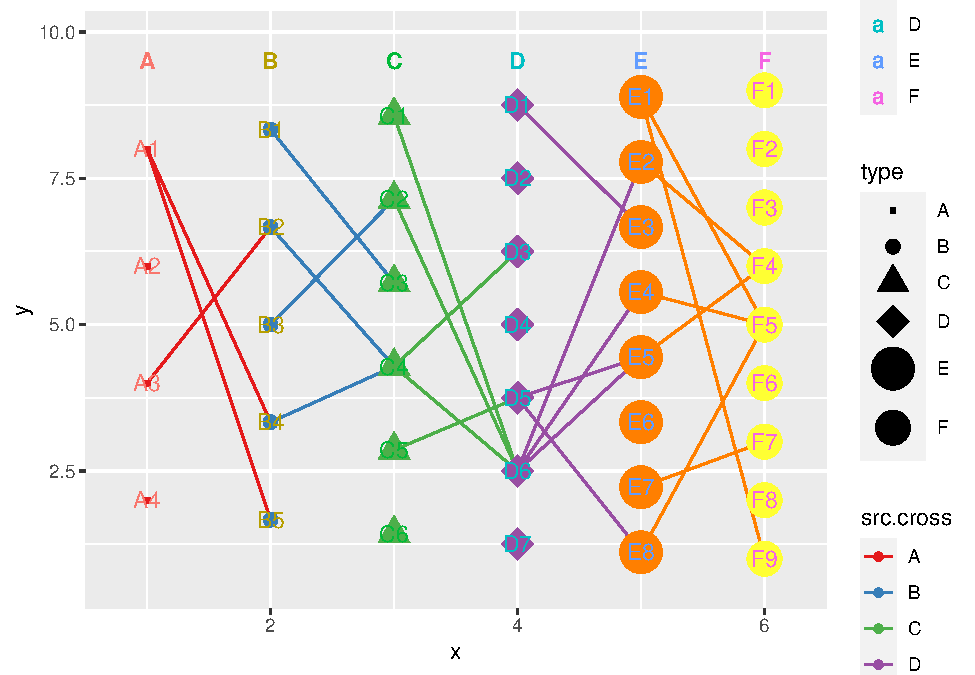
\includegraphics{ReadMe1_files/figure-latex/unnamed-chunk-9-1.pdf}

\begin{Shaded}
\begin{Highlighting}[]
\CommentTok{# set colors, linetypes and size of edges}
\CommentTok{# link: a named list of arguments for links. usage same as ggplot2::geom_segment(). Set NULL to use default settings, or Set NA to not show.}
\NormalTok{cl }\OperatorTok\StringTok{ }\KeywordTok{cl_plot}\NormalTok{( }\DataTypeTok{link =} \KeywordTok{list}\NormalTok{(}\DataTypeTok{mapping =}  \KeywordTok{aes}\NormalTok{(}\DataTypeTok{color =}\NormalTok{ src.cross,}\DataTypeTok{linetype =}\NormalTok{src.cross),}
                            \DataTypeTok{scale   =} \KeywordTok{list}\NormalTok{(}\DataTypeTok{color =} \KeywordTok{scale_color_manual}\NormalTok{(}\DataTypeTok{values =}\NormalTok{ RColorBrewer}\OperatorTok{::}\KeywordTok{brewer.pal}\NormalTok{(}\DecValTok{8}\NormalTok{, }\StringTok{"Set1"}\NormalTok{)),}
                                           \DataTypeTok{linetype =}\KeywordTok{scale_linetype_manual}\NormalTok{(}\DataTypeTok{values =} \KeywordTok{c}\NormalTok{(}\DecValTok{1}\OperatorTok{:}\DecValTok{6}\NormalTok{))),}
                            \DataTypeTok{size    =} \FloatTok{1.5}
\NormalTok{                           ))}
\end{Highlighting}
\end{Shaded}

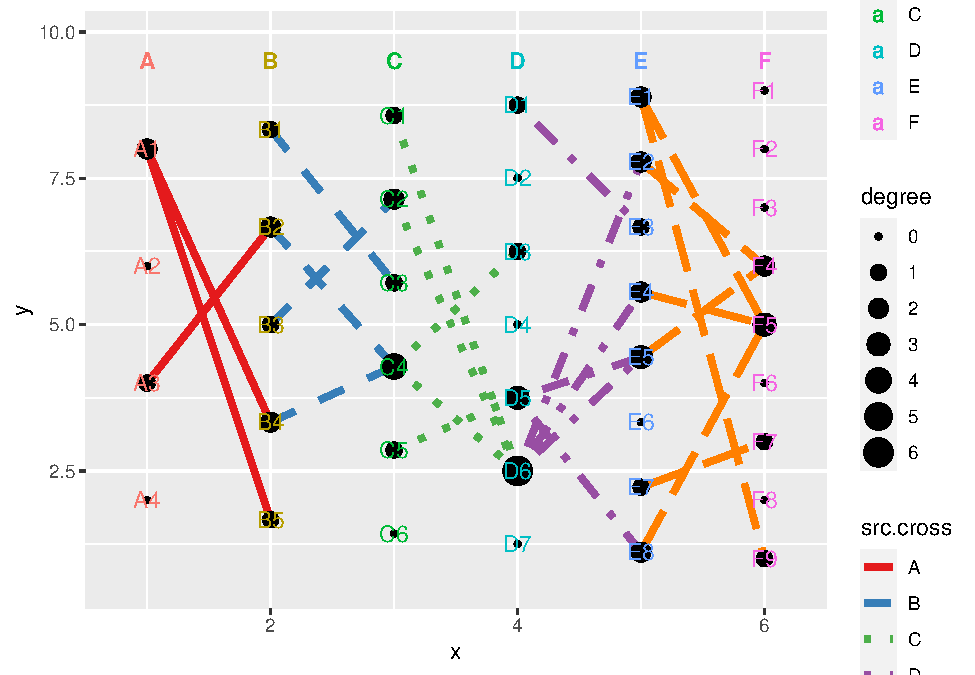
\includegraphics{ReadMe1_files/figure-latex/unnamed-chunk-9-2.pdf}

\begin{Shaded}
\begin{Highlighting}[]
\CommentTok{# set header styles}
\CommentTok{# header:   a named list of arguments for headers. usage same as ggplot2::geom_text(). Set NULL to use default settings, or Set NA to not show.}
\NormalTok{cl }\OperatorTok\StringTok{ }\KeywordTok{cl_plot}\NormalTok{(}\DataTypeTok{header =} \KeywordTok{list}\NormalTok{(}\DataTypeTok{mapping =} \KeywordTok{aes}\NormalTok{(}\DataTypeTok{color=}\NormalTok{ cross),}
                               \DataTypeTok{scale =} \KeywordTok{list}\NormalTok{(}\DataTypeTok{color =} \KeywordTok{scale_color_manual}\NormalTok{(}\DataTypeTok{values =}\NormalTok{ RColorBrewer}\OperatorTok{::}\KeywordTok{brewer.pal}\NormalTok{(}\DecValTok{8}\NormalTok{, }\StringTok{"Dark2"}\NormalTok{))),}
                                \DataTypeTok{size =} \DecValTok{5}
\NormalTok{                             ))}
\end{Highlighting}
\end{Shaded}

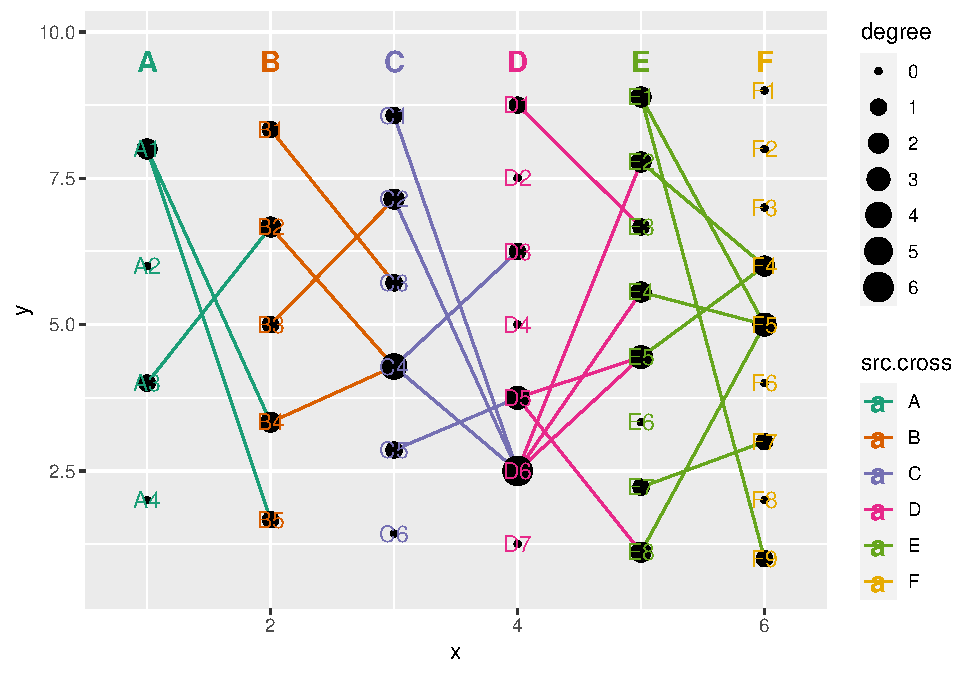
\includegraphics{ReadMe1_files/figure-latex/unnamed-chunk-9-3.pdf}

\begin{Shaded}
\begin{Highlighting}[]
\CommentTok{# set figure theme}
\CommentTok{# add:  other gg object to be added to final plot, such as theme().}
\NormalTok{theme_use <-}\StringTok{ }\KeywordTok{theme}\NormalTok{(}\DataTypeTok{legend.position =} \StringTok{"none"}\NormalTok{,}\DataTypeTok{aspect.ratio =} \DecValTok{1}\NormalTok{,}
                   \DataTypeTok{axis.title =} \KeywordTok{element_blank}\NormalTok{(),}
                   \DataTypeTok{axis.text =} \KeywordTok{element_blank}\NormalTok{(),}
                   \DataTypeTok{axis.ticks =} \KeywordTok{element_blank}\NormalTok{(),}
                   \DataTypeTok{panel.grid =} \KeywordTok{element_blank}\NormalTok{(),}
                   \DataTypeTok{panel.background =} \KeywordTok{element_blank}\NormalTok{())}
\NormalTok{cl }\OperatorTok\StringTok{ }\KeywordTok{cl_plot}\NormalTok{(}\DataTypeTok{add=}\NormalTok{theme_use)}
\end{Highlighting}
\end{Shaded}

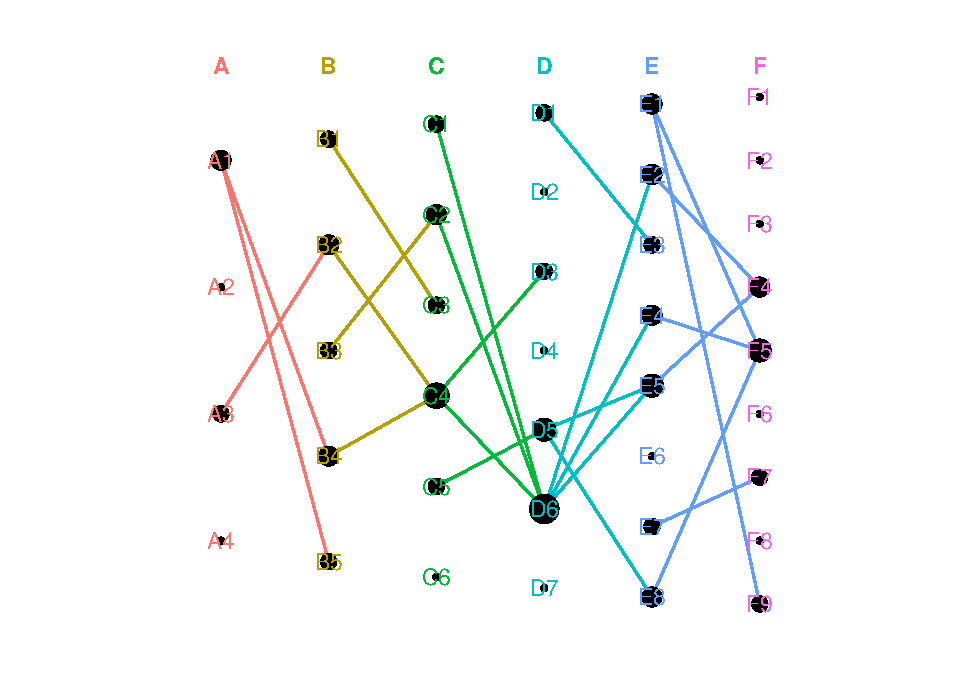
\includegraphics{ReadMe1_files/figure-latex/unnamed-chunk-9-4.pdf}

\hypertarget{c.-annotation-figure}{%
\paragraph{c.~annotation figure}\label{c.-annotation-figure}}

\begin{Shaded}
\begin{Highlighting}[]
\CommentTok{# cl_annotation: add annotation figure. }
\CommentTok{# top, bottom, left or  right   : ggplot object}
\CommentTok{# top.by, bottom.by, left.by, right.by : name of cross by which to align ggplot}

\NormalTok{ann.data <-}\StringTok{ }\KeywordTok{data.frame}\NormalTok{(}\DataTypeTok{F=}\KeywordTok{factor}\NormalTok{(}\KeywordTok{paste0}\NormalTok{(}\StringTok{"F"}\NormalTok{,}\KeywordTok{c}\NormalTok{(}\DecValTok{1}\OperatorTok{:}\DecValTok{10}\NormalTok{)),}\DataTypeTok{levels=}\KeywordTok{paste0}\NormalTok{(}\StringTok{"F"}\NormalTok{,}\KeywordTok{c}\NormalTok{(}\DecValTok{10}\OperatorTok{:}\DecValTok{1}\NormalTok{))),}\DataTypeTok{value=}\KeywordTok{sample}\NormalTok{(}\DataTypeTok{size =} \DecValTok{10}\NormalTok{,}\DataTypeTok{x=}\KeywordTok{c}\NormalTok{(}\DecValTok{1}\OperatorTok{:}\DecValTok{10}\NormalTok{)))}
\NormalTok{ann.data }\OperatorTok\StringTok{ }\KeywordTok{ggplot}\NormalTok{(}\DataTypeTok{mapping =} \KeywordTok{aes}\NormalTok{(}\DataTypeTok{x=}\NormalTok{F,}\DataTypeTok{y=}\NormalTok{value))}\OperatorTok{+}\KeywordTok{geom_bar}\NormalTok{(}\DataTypeTok{stat=}\StringTok{"identity"}\NormalTok{)}\OperatorTok{+}\KeywordTok{coord_flip}\NormalTok{() ->}\StringTok{ }\NormalTok{rgtAnn}

\NormalTok{cl }\OperatorTok\StringTok{ }\KeywordTok{cl_plot}\NormalTok{(}\DataTypeTok{annotation=}\KeywordTok{cl_annotation}\NormalTok{(}\DataTypeTok{right=}\NormalTok{ rgtAnn,}\DataTypeTok{right.by =}\StringTok{"F"}\NormalTok{))}
\end{Highlighting}
\end{Shaded}

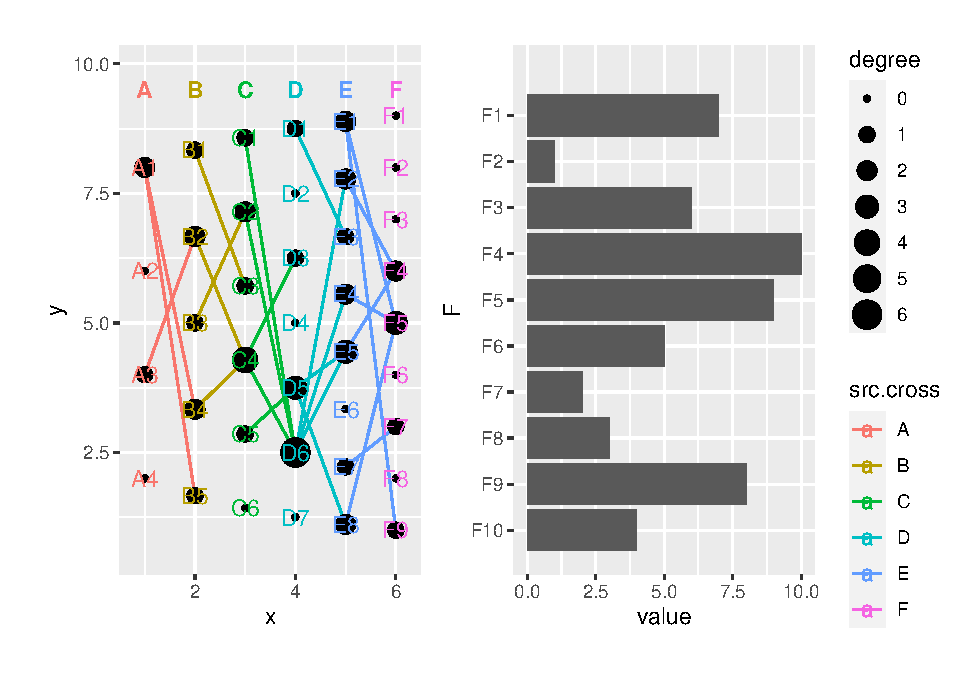
\includegraphics{ReadMe1_files/figure-latex/unnamed-chunk-10-1.pdf}

\hypertarget{examples}{%
\subsection{4. Examples}\label{examples}}

There are examples used in paper and practical application.

\hypertarget{examples-used-in-paper}{%
\subsubsection{1). examples used in
paper}\label{examples-used-in-paper}}

\hypertarget{a.-layout-by-row}{%
\paragraph{a. layout by row}\label{a.-layout-by-row}}

\begin{Shaded}
\begin{Highlighting}[]
\NormalTok{cl <-}\StringTok{ }\KeywordTok{crosslink}\NormalTok{(demo}\OperatorTok{$}\NormalTok{nodes, demo}\OperatorTok{$}\NormalTok{edges, demo}\OperatorTok{$}\NormalTok{cross.by, }\DataTypeTok{odd.rm =}\NormalTok{ F,}\DataTypeTok{spaces =} \StringTok{"flank"}\NormalTok{)}

\NormalTok{cl }\OperatorTok\StringTok{ }\KeywordTok{layout_row}\NormalTok{() }\OperatorTok
\StringTok{   }\KeywordTok{cl_plot}\NormalTok{(}\DataTypeTok{cross =} \KeywordTok{list}\NormalTok{(}\DataTypeTok{mapping =} \KeywordTok{aes}\NormalTok{(}\DataTypeTok{color  =}\NormalTok{ type,}\DataTypeTok{fill=}\NormalTok{type),}
                        \DataTypeTok{scale   =} \KeywordTok{list}\NormalTok{(}\DataTypeTok{color =} \KeywordTok{scale_color_manual}\NormalTok{(}\DataTypeTok{values =}\NormalTok{ RColorBrewer}\OperatorTok{::}\KeywordTok{brewer.pal}\NormalTok{(}\DecValTok{8}\NormalTok{, }\StringTok{"Dark2"}\NormalTok{)),}
                                        \DataTypeTok{fill =} \KeywordTok{scale_fill_manual}\NormalTok{( }\DataTypeTok{values =}\NormalTok{ RColorBrewer}\OperatorTok{::}\KeywordTok{brewer.pal}\NormalTok{(}\DecValTok{8}\NormalTok{, }\StringTok{"Dark2"}\NormalTok{))),}
                        \DataTypeTok{size=}\DecValTok{8}\NormalTok{,}\DataTypeTok{shape=}\DecValTok{24}
\NormalTok{                       ),}
          \DataTypeTok{link   =} \KeywordTok{list}\NormalTok{(}\DataTypeTok{color=}\NormalTok{RColorBrewer}\OperatorTok{::}\KeywordTok{brewer.pal}\NormalTok{(}\DecValTok{8}\NormalTok{, }\StringTok{"Set2"}\NormalTok{)[}\DecValTok{7}\NormalTok{],}\DataTypeTok{size=}\FloatTok{1.5}\NormalTok{,}\DataTypeTok{linetype=}\DecValTok{12}\NormalTok{),}
          \DataTypeTok{label  =} \KeywordTok{list}\NormalTok{(}\DataTypeTok{color=}\StringTok{"white"}\NormalTok{),}
          \DataTypeTok{header =} \KeywordTok{list}\NormalTok{(}\DataTypeTok{mapping =} \KeywordTok{aes}\NormalTok{(}\DataTypeTok{color=}\NormalTok{ cross),}
                        \DataTypeTok{scale =} \KeywordTok{list}\NormalTok{(}\DataTypeTok{color =} \KeywordTok{scale_color_manual}\NormalTok{(}\DataTypeTok{values =}\NormalTok{ RColorBrewer}\OperatorTok{::}\KeywordTok{brewer.pal}\NormalTok{(}\DecValTok{8}\NormalTok{, }\StringTok{"Dark2"}\NormalTok{))),}
                        \DataTypeTok{size=}\DecValTok{5}
\NormalTok{                       ),}
          \DataTypeTok{add=}\NormalTok{theme_use)}
\end{Highlighting}
\end{Shaded}

\begin{verbatim}
## Copy layout default into default, and Set active layout to default
\end{verbatim}

\begin{verbatim}
## Copy layout temp into default, and Set active layout to default
\end{verbatim}

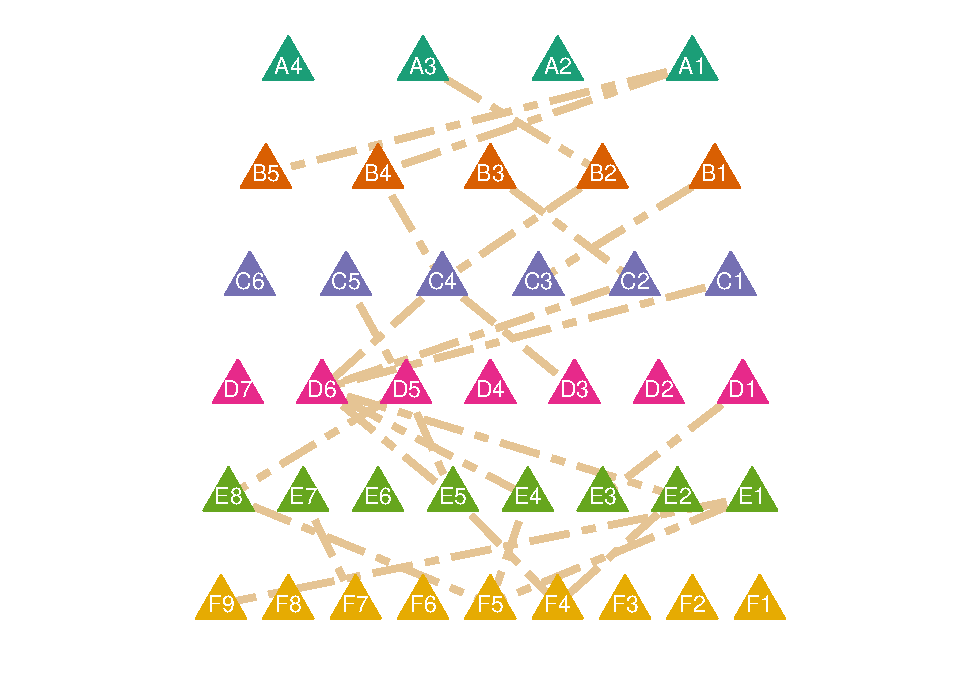
\includegraphics{ReadMe1_files/figure-latex/unnamed-chunk-11-1.pdf}

\hypertarget{b.-layout-by-rotate}{%
\paragraph{b. layout by rotate}\label{b.-layout-by-rotate}}

\begin{Shaded}
\begin{Highlighting}[]
\NormalTok{cl }\OperatorTok\StringTok{ }
\StringTok{   }\KeywordTok{tf_rotate}\NormalTok{(}\DataTypeTok{angle =} \DecValTok{15}\NormalTok{, }\DataTypeTok{by.each.cross =}\NormalTok{ T) }\OperatorTok
\StringTok{   }\KeywordTok{cl_plot}\NormalTok{(}\DataTypeTok{cross =} \KeywordTok{list}\NormalTok{(}\DataTypeTok{mapping =} \KeywordTok{aes}\NormalTok{(}\DataTypeTok{color =}\NormalTok{ type),}
                       \DataTypeTok{scale =} \KeywordTok{list}\NormalTok{(}\DataTypeTok{color =} \KeywordTok{scale_color_manual}\NormalTok{(}\DataTypeTok{values =}\NormalTok{ RColorBrewer}\OperatorTok{::}\KeywordTok{brewer.pal}\NormalTok{(}\DecValTok{8}\NormalTok{, }\StringTok{"Dark2"}\NormalTok{))),}
                       \DataTypeTok{size=}\DecValTok{10}\NormalTok{,}\DataTypeTok{shape=}\DecValTok{16}
\NormalTok{                       ),}
          \DataTypeTok{link =} \KeywordTok{list}\NormalTok{(}\DataTypeTok{color=}\StringTok{"grey75"}\NormalTok{,}\DataTypeTok{size=}\DecValTok{1}\NormalTok{,}\DataTypeTok{linetype=}\DecValTok{15}\NormalTok{),}
          \DataTypeTok{label =} \KeywordTok{list}\NormalTok{(}\DataTypeTok{color=}\StringTok{"white"}\NormalTok{),}
          \DataTypeTok{header =} \KeywordTok{list}\NormalTok{(}\DataTypeTok{mapping =} \KeywordTok{aes}\NormalTok{(}\DataTypeTok{color=}\NormalTok{ cross),}
                       \DataTypeTok{scale =} \KeywordTok{list}\NormalTok{(}\DataTypeTok{color =} \KeywordTok{scale_color_manual}\NormalTok{(}\DataTypeTok{values =}\NormalTok{ RColorBrewer}\OperatorTok{::}\KeywordTok{brewer.pal}\NormalTok{(}\DecValTok{8}\NormalTok{, }\StringTok{"Dark2"}\NormalTok{))),}
                       \DataTypeTok{size=}\DecValTok{5}
\NormalTok{                       ),}
          \DataTypeTok{add=}\NormalTok{theme_use)}
\end{Highlighting}
\end{Shaded}

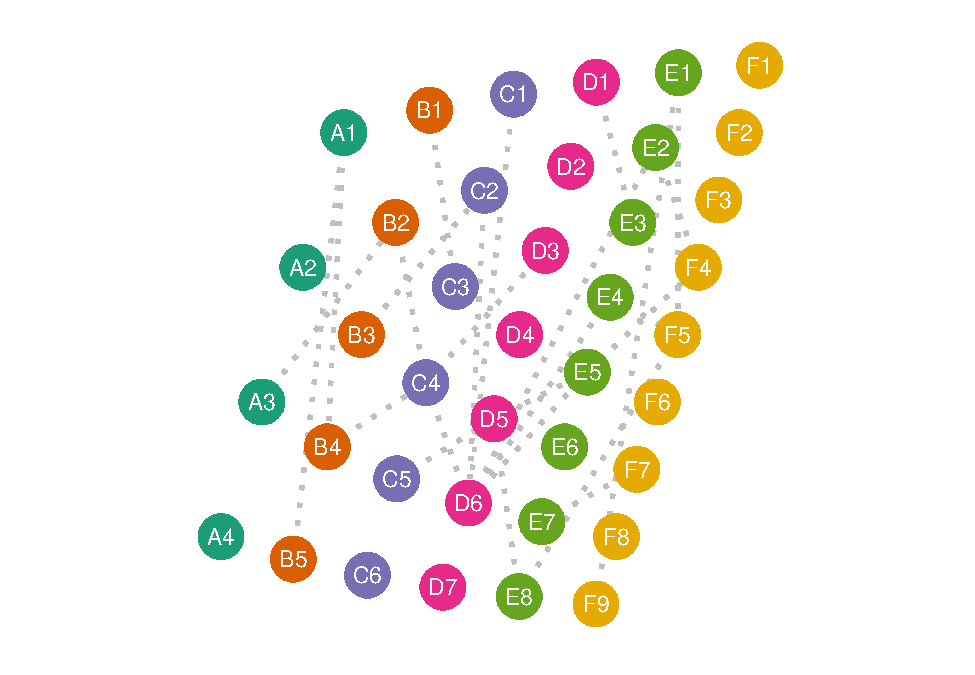
\includegraphics{ReadMe1_files/figure-latex/unnamed-chunk-12-1.pdf}

\hypertarget{c.-layout-by-polygon}{%
\paragraph{c.~layout by polygon}\label{c.-layout-by-polygon}}

\begin{Shaded}
\begin{Highlighting}[]
\NormalTok{cl }\OperatorTok\StringTok{ }\KeywordTok{layout_polygon}\NormalTok{() }\OperatorTok
\StringTok{   }\CommentTok{#tf_rotate(angle = 45, by.each.cross = F) %>%  # If the grouping is 4, rotate by this parameter and change from diamond to square }
\StringTok{   }\KeywordTok{cl_plot}\NormalTok{(}\DataTypeTok{cross =} \KeywordTok{list}\NormalTok{(}\DataTypeTok{mapping =} \KeywordTok{aes}\NormalTok{(}\DataTypeTok{color =}\NormalTok{ type),}
                        \DataTypeTok{scale =} \KeywordTok{list}\NormalTok{(}\DataTypeTok{color =} \KeywordTok{scale_color_manual}\NormalTok{(}\DataTypeTok{values =}\NormalTok{ RColorBrewer}\OperatorTok{::}\KeywordTok{brewer.pal}\NormalTok{(}\DecValTok{8}\NormalTok{, }\StringTok{"Dark2"}\NormalTok{))),}
                        \DataTypeTok{size=}\DecValTok{10}\NormalTok{,}\DataTypeTok{shape=}\DecValTok{16}
\NormalTok{                       ),}
           \DataTypeTok{link  =} \KeywordTok{list}\NormalTok{(}\DataTypeTok{color=}\StringTok{"orange"}\NormalTok{,}\DataTypeTok{size=}\DecValTok{2}\NormalTok{,}\DataTypeTok{linetype=}\DecValTok{15}\NormalTok{,}\DataTypeTok{geom=}\StringTok{"curve"}\NormalTok{),}
           \DataTypeTok{label =} \KeywordTok{list}\NormalTok{(}\DataTypeTok{color=}\StringTok{"white"}\NormalTok{),}
           \DataTypeTok{header=} \KeywordTok{list}\NormalTok{(}\DataTypeTok{mapping =} \KeywordTok{aes}\NormalTok{(}\DataTypeTok{color=}\NormalTok{ cross),}
                        \DataTypeTok{scale =} \KeywordTok{list}\NormalTok{(}\DataTypeTok{color =} \KeywordTok{scale_color_manual}\NormalTok{(}\DataTypeTok{values =}\NormalTok{ RColorBrewer}\OperatorTok{::}\KeywordTok{brewer.pal}\NormalTok{(}\DecValTok{8}\NormalTok{, }\StringTok{"Dark2"}\NormalTok{))),}
                        \DataTypeTok{size=}\DecValTok{5}
\NormalTok{                        ),}
           \DataTypeTok{add  =}\NormalTok{  theme_use )}
\end{Highlighting}
\end{Shaded}

\begin{verbatim}
## Copy layout default into default, and Set active layout to default
\end{verbatim}

\begin{verbatim}
## Copy layout temp into default, and Set active layout to default
\end{verbatim}

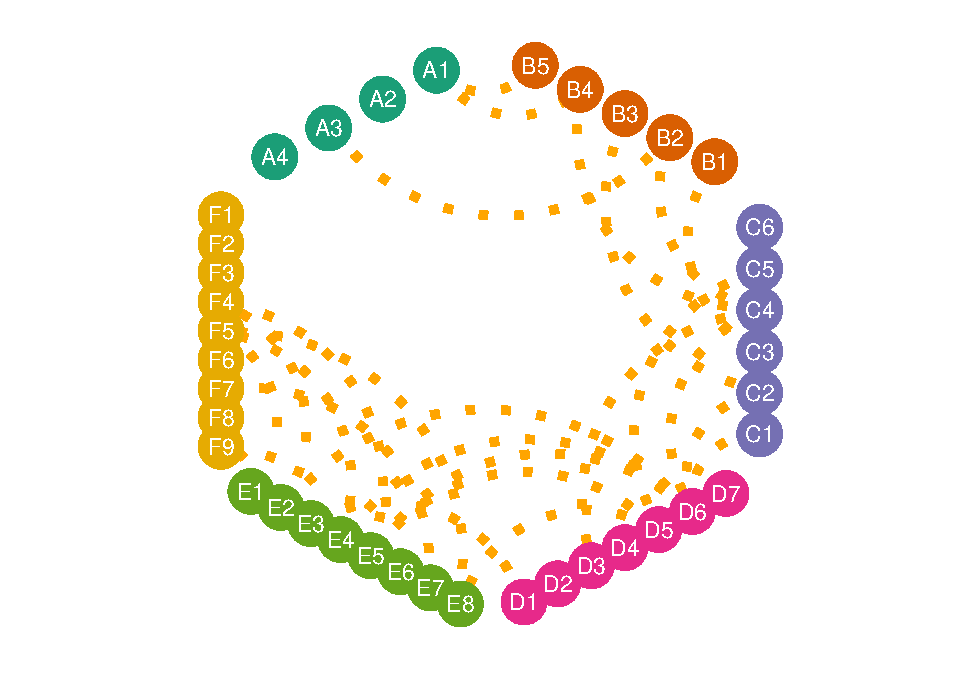
\includegraphics{ReadMe1_files/figure-latex/unnamed-chunk-13-1.pdf}

\hypertarget{d.-layout-by-hive}{%
\paragraph{d.~layout by hive}\label{d.-layout-by-hive}}

\begin{Shaded}
\begin{Highlighting}[]
\NormalTok{cl }\OperatorTok\StringTok{ }\KeywordTok{layout_hive}\NormalTok{(}\DataTypeTok{angles=}\KeywordTok{rep}\NormalTok{(}\DecValTok{60}\NormalTok{,}\DecValTok{6}\NormalTok{)) }\OperatorTok\StringTok{ }\CommentTok{#length of angles must be same with the numbers of groups}
\StringTok{       }\KeywordTok{cl_plot}\NormalTok{(}\DataTypeTok{cross =} \KeywordTok{list}\NormalTok{(}\DataTypeTok{mapping =} \KeywordTok{aes}\NormalTok{(}\DataTypeTok{color =}\NormalTok{ type),}
                       \DataTypeTok{scale =} \KeywordTok{list}\NormalTok{(}\DataTypeTok{color =} \KeywordTok{scale_color_manual}\NormalTok{(}\DataTypeTok{values =}\NormalTok{ RColorBrewer}\OperatorTok{::}\KeywordTok{brewer.pal}\NormalTok{(}\DecValTok{8}\NormalTok{, }\StringTok{"Dark2"}\NormalTok{))),}
                       \DataTypeTok{size=}\DecValTok{10}\NormalTok{,}\DataTypeTok{shape=}\DecValTok{18}
\NormalTok{                       ),}
               \DataTypeTok{link  =} \KeywordTok{list}\NormalTok{(}\DataTypeTok{color=}\StringTok{"purple"}\NormalTok{,}\DataTypeTok{size=}\DecValTok{1}\NormalTok{,}\DataTypeTok{linetype=}\DecValTok{15}\NormalTok{),}
               \DataTypeTok{label =} \KeywordTok{list}\NormalTok{(}\DataTypeTok{color=}\StringTok{"white"}\NormalTok{),}
               \DataTypeTok{header=} \KeywordTok{list}\NormalTok{(}\DataTypeTok{mapping =} \KeywordTok{aes}\NormalTok{(}\DataTypeTok{color=}\NormalTok{ cross),}
                            \DataTypeTok{scale =} \KeywordTok{list}\NormalTok{(}\DataTypeTok{color =} \KeywordTok{scale_color_manual}\NormalTok{(}\DataTypeTok{values =}\NormalTok{ RColorBrewer}\OperatorTok{::}\KeywordTok{brewer.pal}\NormalTok{(}\DecValTok{8}\NormalTok{, }\StringTok{"Dark2"}\NormalTok{))),}
                            \DataTypeTok{size=}\DecValTok{5}
\NormalTok{                            ),}
               \DataTypeTok{add   =}\NormalTok{ theme_use )}
\end{Highlighting}
\end{Shaded}

\begin{verbatim}
## Copy layout default into default, and Set active layout to default
\end{verbatim}

\begin{verbatim}
## Copy layout temp into default, and Set active layout to default
\end{verbatim}

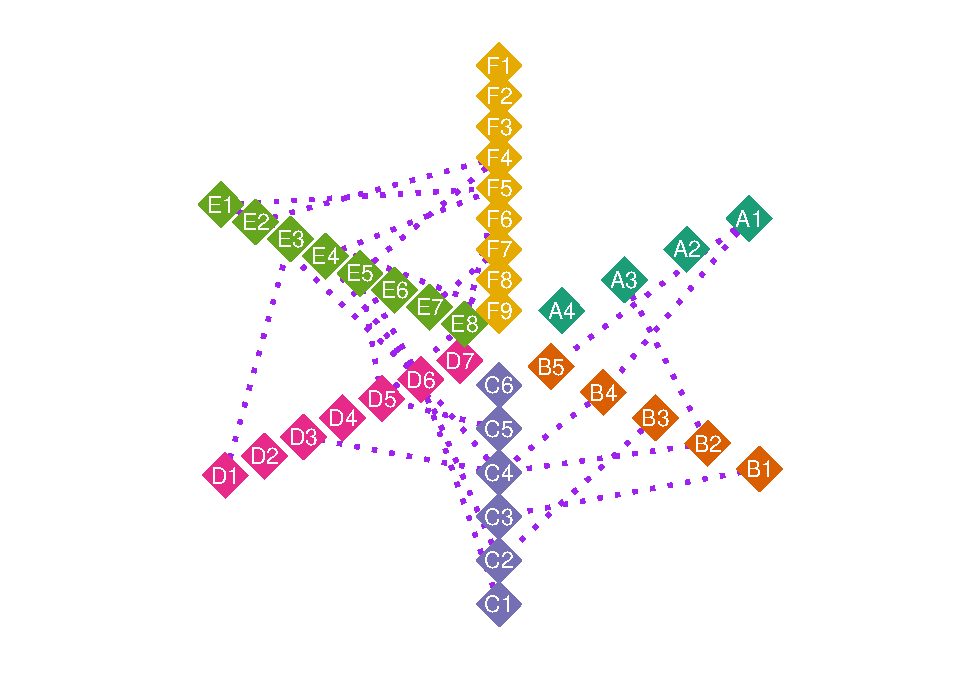
\includegraphics{ReadMe1_files/figure-latex/unnamed-chunk-14-1.pdf}

\hypertarget{e.-layout-by-arc}{%
\paragraph{e. layout by arc}\label{e.-layout-by-arc}}

\begin{Shaded}
\begin{Highlighting}[]
\NormalTok{cl }\OperatorTok\StringTok{ }\KeywordTok{layout_arc}\NormalTok{(}\DataTypeTok{angles=}\KeywordTok{c}\NormalTok{(}\DecValTok{60}\NormalTok{,}\DecValTok{120}\NormalTok{,}\DecValTok{180}\NormalTok{),}\DataTypeTok{crosses=}\KeywordTok{c}\NormalTok{(}\StringTok{"D"}\NormalTok{,}\StringTok{"E"}\NormalTok{,}\StringTok{"F"}\NormalTok{)) }\OperatorTok\StringTok{ }\CommentTok{#length of angles must be same with the numbers of crosses}
\StringTok{       }\KeywordTok{cl_plot}\NormalTok{(}\DataTypeTok{cross =} \KeywordTok{list}\NormalTok{(}\DataTypeTok{mapping =} \KeywordTok{aes}\NormalTok{(}\DataTypeTok{color =}\NormalTok{ type),}
                            \DataTypeTok{scale =} \KeywordTok{list}\NormalTok{(}\DataTypeTok{color =} \KeywordTok{scale_color_manual}\NormalTok{(}\DataTypeTok{values =}\NormalTok{ RColorBrewer}\OperatorTok{::}\KeywordTok{brewer.pal}\NormalTok{(}\DecValTok{8}\NormalTok{, }\StringTok{"Dark2"}\NormalTok{))),}
                            \DataTypeTok{size=}\DecValTok{10}\NormalTok{,}\DataTypeTok{shape=}\DecValTok{18}
\NormalTok{                           ),}
               \DataTypeTok{link  =} \KeywordTok{list}\NormalTok{(}\DataTypeTok{color=}\StringTok{"orange"}\NormalTok{,}\DataTypeTok{size=}\DecValTok{1}\NormalTok{,}\DataTypeTok{linetype=}\DecValTok{3}\NormalTok{),}\CommentTok{#,geom="curve"}
               \DataTypeTok{label =} \KeywordTok{list}\NormalTok{(}\DataTypeTok{color=}\StringTok{"white"}\NormalTok{),}
               \DataTypeTok{header=} \KeywordTok{list}\NormalTok{(}\DataTypeTok{mapping =} \KeywordTok{aes}\NormalTok{(}\DataTypeTok{color=}\NormalTok{ cross),}
                            \DataTypeTok{scale =} \KeywordTok{list}\NormalTok{(}\DataTypeTok{color =} \KeywordTok{scale_color_manual}\NormalTok{(}\DataTypeTok{values =}\NormalTok{ RColorBrewer}\OperatorTok{::}\KeywordTok{brewer.pal}\NormalTok{(}\DecValTok{8}\NormalTok{, }\StringTok{"Dark2"}\NormalTok{))),}
                            \DataTypeTok{size=}\DecValTok{5}
\NormalTok{                           ),}
               \DataTypeTok{add   =}\NormalTok{  theme_use)}
\end{Highlighting}
\end{Shaded}

\begin{verbatim}
## Copy layout default into temp, and Set active layout to temp
\end{verbatim}

\begin{verbatim}
## Copy layout default into default, and Set active layout to default
\end{verbatim}

\begin{verbatim}
## Copy layout temp into default, and Set active layout to default
\end{verbatim}

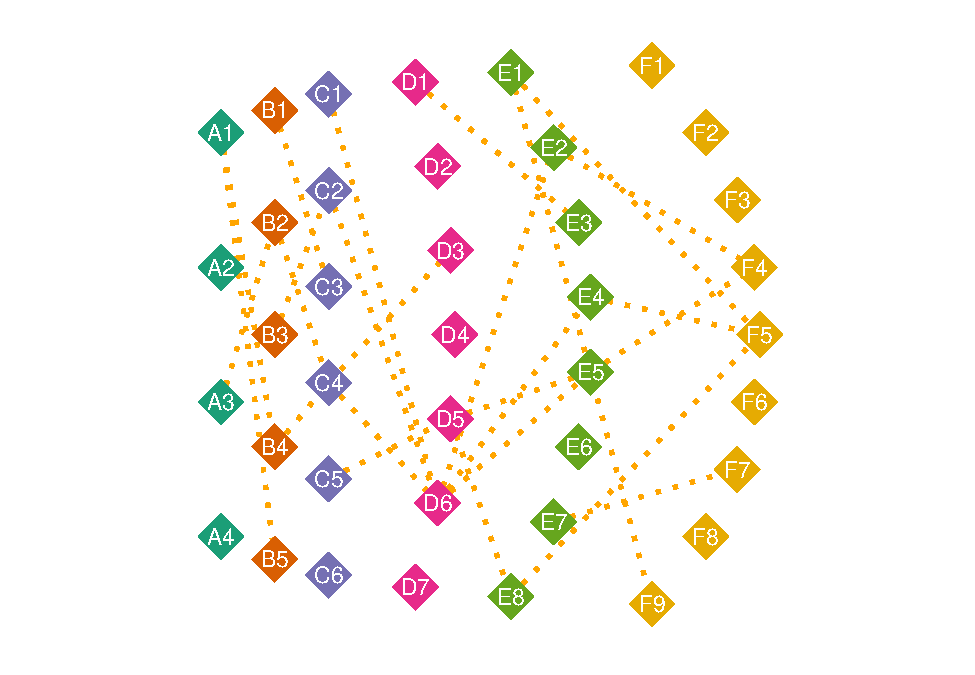
\includegraphics{ReadMe1_files/figure-latex/unnamed-chunk-15-1.pdf}

\hypertarget{f.-layout-by-combination-of-several-methods}{%
\paragraph{f.~layout by combination of several
methods}\label{f.-layout-by-combination-of-several-methods}}

\begin{Shaded}
\begin{Highlighting}[]
\CommentTok{# demo data}
\NormalTok{n <-}\StringTok{ }\DecValTok{5}
\NormalTok{demo <-}\StringTok{ }\KeywordTok{gen_demo}\NormalTok{(}\DataTypeTok{n_cross =}\NormalTok{ n, }\DataTypeTok{n_node =} \KeywordTok{rep}\NormalTok{(n, n), }\DataTypeTok{n_link =} \KeywordTok{rep}\NormalTok{(n, n}\DecValTok{-1}\NormalTok{), }\DataTypeTok{seed =} \DecValTok{66}\NormalTok{)}
\NormalTok{nodes <-}\StringTok{ }\NormalTok{demo}\OperatorTok{$}\NormalTok{nodes}
\NormalTok{edges <-}\StringTok{ }\NormalTok{demo}\OperatorTok{$}\NormalTok{edges}
\NormalTok{cross.by <-}\StringTok{ }\NormalTok{demo}\OperatorTok{$}\NormalTok{cross.by}


\NormalTok{cl <-}\StringTok{ }\KeywordTok{crosslink}\NormalTok{(nodes, edges, cross.by, }\DataTypeTok{odd.rm =}\NormalTok{ F)}
\NormalTok{cl <-}\StringTok{ }\KeywordTok{set_header}\NormalTok{(cl,}\DataTypeTok{header =} \KeywordTok{c}\NormalTok{(}\StringTok{"A"}\NormalTok{,}\StringTok{"B"}\NormalTok{,}\StringTok{"C"}\NormalTok{,}\StringTok{"D"}\NormalTok{,}\StringTok{"E"}\NormalTok{))}

\NormalTok{cl }\OperatorTok\StringTok{ }
\StringTok{   }\KeywordTok{layout_polygon}\NormalTok{(}\DataTypeTok{crosses =} \KeywordTok{c}\NormalTok{(}\StringTok{"A"}\NormalTok{,}\StringTok{"B"}\NormalTok{,}\StringTok{"C"}\NormalTok{,}\StringTok{"D"}\NormalTok{)) }\OperatorTok
\StringTok{   }\KeywordTok{tf_rotate}\NormalTok{(}\DataTypeTok{crosses=}\KeywordTok{c}\NormalTok{(}\StringTok{"A"}\NormalTok{,}\StringTok{"B"}\NormalTok{,}\StringTok{"C"}\NormalTok{,}\StringTok{"D"}\NormalTok{),}\DataTypeTok{angle =} \KeywordTok{rep}\NormalTok{(}\DecValTok{45}\NormalTok{,}\DecValTok{4}\NormalTok{)) }\OperatorTok
\StringTok{   }\KeywordTok{tf_shift}\NormalTok{(}\DataTypeTok{x=}\FloatTok{0.8}\OperatorTok{*}\NormalTok{(}\OperatorTok{-}\DecValTok{1}\NormalTok{),}\DataTypeTok{y=}\FloatTok{0.05}\NormalTok{,}\DataTypeTok{crosses=}\StringTok{"E"}\NormalTok{,}\DataTypeTok{layout=}\StringTok{"default"}\NormalTok{) ->cl}
\end{Highlighting}
\end{Shaded}

\begin{verbatim}
## Copy layout default into default, and Set active layout to default
\end{verbatim}

\begin{verbatim}
## Copy layout temp into default, and Set active layout to default
\end{verbatim}

\begin{Shaded}
\begin{Highlighting}[]
\NormalTok{cl }\OperatorTok
\StringTok{   }\KeywordTok{cl_plot}\NormalTok{(}\DataTypeTok{cross =} \KeywordTok{list}\NormalTok{(}\DataTypeTok{mapping =} \KeywordTok{aes}\NormalTok{(}\DataTypeTok{color =}\NormalTok{ type),}
                       \DataTypeTok{scale =} \KeywordTok{list}\NormalTok{(}\DataTypeTok{color =} \KeywordTok{scale_color_manual}\NormalTok{(}\DataTypeTok{values =}\NormalTok{ RColorBrewer}\OperatorTok{::}\KeywordTok{brewer.pal}\NormalTok{(}\DecValTok{8}\NormalTok{, }\StringTok{"Dark2"}\NormalTok{))),}
                       \DataTypeTok{size=}\DecValTok{10}\NormalTok{,}\DataTypeTok{shape=}\DecValTok{19}
\NormalTok{                       ),}
          \DataTypeTok{link   =} \KeywordTok{list}\NormalTok{(}\DataTypeTok{color=}\StringTok{"grey75"}\NormalTok{,}\DataTypeTok{size=}\DecValTok{1}\NormalTok{,}\DataTypeTok{linetype=}\DecValTok{3}\NormalTok{),}
          \DataTypeTok{label  =} \KeywordTok{list}\NormalTok{(}\DataTypeTok{color=}\StringTok{"white"}\NormalTok{),}
          \DataTypeTok{header =} \KeywordTok{list}\NormalTok{(}\DataTypeTok{mapping =} \KeywordTok{aes}\NormalTok{(}\DataTypeTok{color=}\NormalTok{ cross),}
                       \DataTypeTok{scale =} \KeywordTok{list}\NormalTok{(}\DataTypeTok{color =} \KeywordTok{scale_color_manual}\NormalTok{(}\DataTypeTok{values =}\NormalTok{ RColorBrewer}\OperatorTok{::}\KeywordTok{brewer.pal}\NormalTok{(}\DecValTok{8}\NormalTok{, }\StringTok{"Dark2"}\NormalTok{))),}
                       \DataTypeTok{size=}\DecValTok{5}
\NormalTok{                       ),}
           \DataTypeTok{add   =}\NormalTok{  theme_use)}
\end{Highlighting}
\end{Shaded}

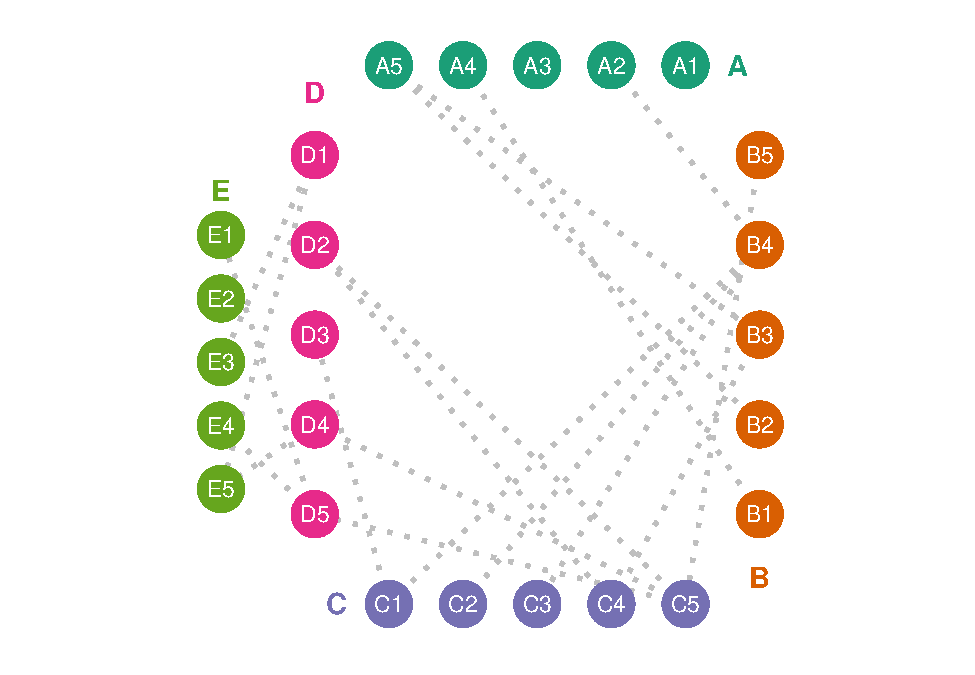
\includegraphics{ReadMe1_files/figure-latex/unnamed-chunk-16-1.pdf}

\hypertarget{examples-of-complex-figure}{%
\subsubsection{2). examples of complex
figure}\label{examples-of-complex-figure}}

\begin{Shaded}
\begin{Highlighting}[]
\KeywordTok{library}\NormalTok{(dplyr)}
\end{Highlighting}
\end{Shaded}

\begin{verbatim}
## 
## Attaching package: 'dplyr'
\end{verbatim}

\begin{verbatim}
## The following objects are masked from 'package:stats':
## 
##     filter, lag
\end{verbatim}

\begin{verbatim}
## The following objects are masked from 'package:base':
## 
##     intersect, setdiff, setequal, union
\end{verbatim}

\begin{Shaded}
\begin{Highlighting}[]
\KeywordTok{library}\NormalTok{(reshape)}
\end{Highlighting}
\end{Shaded}

\begin{verbatim}
## 
## Attaching package: 'reshape'
\end{verbatim}

\begin{verbatim}
## The following object is masked from 'package:dplyr':
## 
##     rename
\end{verbatim}

\begin{Shaded}
\begin{Highlighting}[]
\KeywordTok{theme_classic}\NormalTok{() }\OperatorTok{+}
\StringTok{  }\KeywordTok{theme}\NormalTok{(}\DataTypeTok{axis.text =} \KeywordTok{element_blank}\NormalTok{(),}
        \DataTypeTok{axis.line.x =} \KeywordTok{element_blank}\NormalTok{(),}
        \DataTypeTok{axis.ticks.x =} \KeywordTok{element_blank}\NormalTok{()) ->theme_use2}


\CommentTok{## crosslink project}
\NormalTok{cl <-}\StringTok{ }\KeywordTok{crosslink}\NormalTok{(example}\OperatorTok{$}\NormalTok{nodes,example}\OperatorTok{$}\NormalTok{edges,}\DataTypeTok{cross.by=}\StringTok{"type"}\NormalTok{)}

\NormalTok{cl }\OperatorTok\StringTok{ }\KeywordTok{cl_plot}\NormalTok{()}
\end{Highlighting}
\end{Shaded}

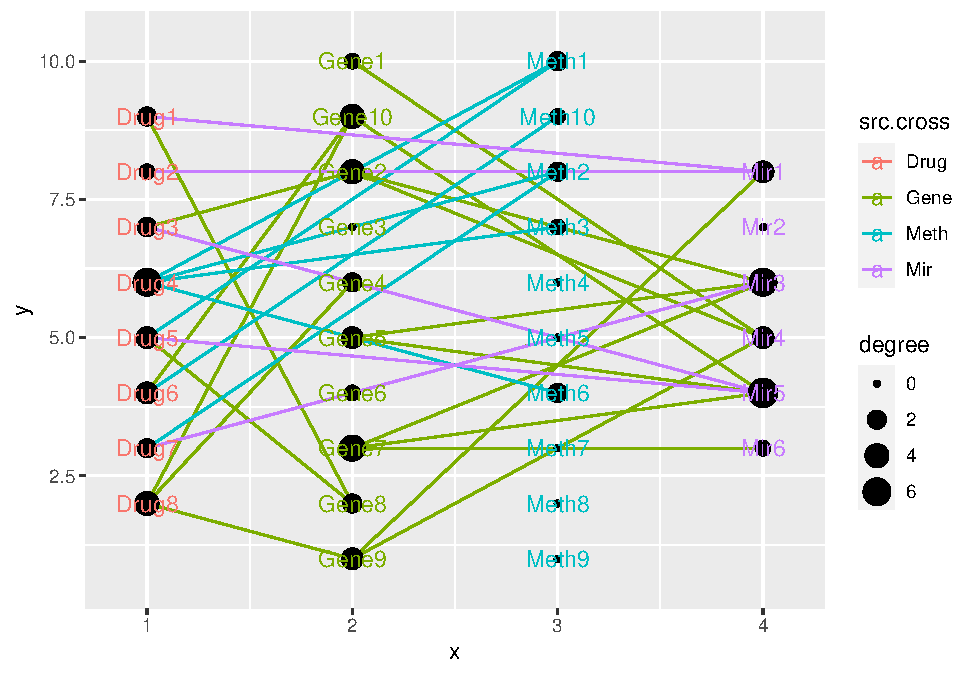
\includegraphics{ReadMe1_files/figure-latex/unnamed-chunk-17-1.pdf}

\begin{Shaded}
\begin{Highlighting}[]
\NormalTok{cl <-}\StringTok{ }\KeywordTok{set_header}\NormalTok{(cl,}\DataTypeTok{header=}\KeywordTok{unique}\NormalTok{(}\KeywordTok{get_cross}\NormalTok{(cl)}\OperatorTok{$}\NormalTok{cross))}

\NormalTok{cl }\OperatorTok\StringTok{ }\KeywordTok{layout_polygon}\NormalTok{(}\DataTypeTok{crosses =} \KeywordTok{c}\NormalTok{(}\StringTok{"Mir"}\NormalTok{,}\StringTok{"Meth"}\NormalTok{,}\StringTok{"Gene"}\NormalTok{,}\StringTok{"Drug"}\NormalTok{),}\DataTypeTok{layout_based =} \StringTok{"default"}\NormalTok{) }\OperatorTok
\StringTok{       }\KeywordTok{tf_rotate}\NormalTok{(}\DataTypeTok{crosses=} \KeywordTok{c}\NormalTok{(}\StringTok{"Mir"}\NormalTok{,}\StringTok{"Meth"}\NormalTok{,}\StringTok{"Gene"}\NormalTok{,}\StringTok{"Drug"}\NormalTok{),}\DataTypeTok{angle =} \KeywordTok{rep}\NormalTok{(}\DecValTok{45}\NormalTok{,}\DecValTok{4}\NormalTok{),}\DataTypeTok{layout=}\StringTok{"default"}\NormalTok{) }\OperatorTok
\StringTok{       }\KeywordTok{tf_shift}\NormalTok{(}\DataTypeTok{x=}\FloatTok{0.2}\OperatorTok{*}\NormalTok{(}\OperatorTok{-}\DecValTok{1}\NormalTok{),}\DataTypeTok{y=}\FloatTok{1.5}\NormalTok{,}\DataTypeTok{crosses=}\KeywordTok{c}\NormalTok{(}\StringTok{"Mir"}\NormalTok{,}\StringTok{"Meth"}\NormalTok{),}\DataTypeTok{layout=}\StringTok{"default"}\NormalTok{) ->}\StringTok{ }\NormalTok{cl}
\end{Highlighting}
\end{Shaded}

\begin{verbatim}
## Copy layout default into default, and Set active layout to default
\end{verbatim}

\begin{verbatim}
## Copy layout temp into default, and Set active layout to default
\end{verbatim}

\begin{Shaded}
\begin{Highlighting}[]
\CommentTok{# plot annotation}
\NormalTok{top <-}\StringTok{ }\NormalTok{nodes}\OperatorTok{$}\NormalTok{id[nodes}\OperatorTok{$}\NormalTok{type }\OperatorTok{==}\StringTok{ "Mir"}\NormalTok{] }\CommentTok{# set the order as you like}
\NormalTok{bottom <-}\StringTok{ }\NormalTok{nodes}\OperatorTok{$}\NormalTok{id[nodes}\OperatorTok{$}\NormalTok{type }\OperatorTok{==}\StringTok{ "Gene"}\NormalTok{] }\CommentTok{# set the order as you like}
\NormalTok{right <-}\StringTok{ }\NormalTok{nodes}\OperatorTok{$}\NormalTok{id[nodes}\OperatorTok{$}\NormalTok{type }\OperatorTok{==}\StringTok{ "Meth"}\NormalTok{] }\CommentTok{# set the order as you like}

\CommentTok{# Top plot}
\NormalTok{topAnn <-}\StringTok{  }\NormalTok{mirData }\OperatorTok
\StringTok{  }\KeywordTok{mutate}\NormalTok{(}\DataTypeTok{mir_f =} \KeywordTok{factor}\NormalTok{(mir, top)) }\OperatorTok
\StringTok{  }\KeywordTok{ggplot}\NormalTok{(}\DataTypeTok{mapping =} \KeywordTok{aes}\NormalTok{(}\DataTypeTok{x=}\NormalTok{mir,}\DataTypeTok{y=}\OperatorTok{-}\NormalTok{lfc)) }\OperatorTok{+}
\StringTok{  }\KeywordTok{geom_bar}\NormalTok{(}\DataTypeTok{fill =} \StringTok{"#E7298A"}\NormalTok{,}
           \DataTypeTok{stat =} \StringTok{"identity"}\NormalTok{,}
           \DataTypeTok{width =} \FloatTok{0.5}\NormalTok{) }\OperatorTok{+}\StringTok{ }
\StringTok{  }\KeywordTok{labs}\NormalTok{(}\DataTypeTok{x =} \OtherTok{NULL}\NormalTok{, }\DataTypeTok{y =} \StringTok{"log2(Fold Change)"}\NormalTok{) }\OperatorTok{+}
\StringTok{  }\NormalTok{theme_use2}
\NormalTok{topAnn}
\end{Highlighting}
\end{Shaded}

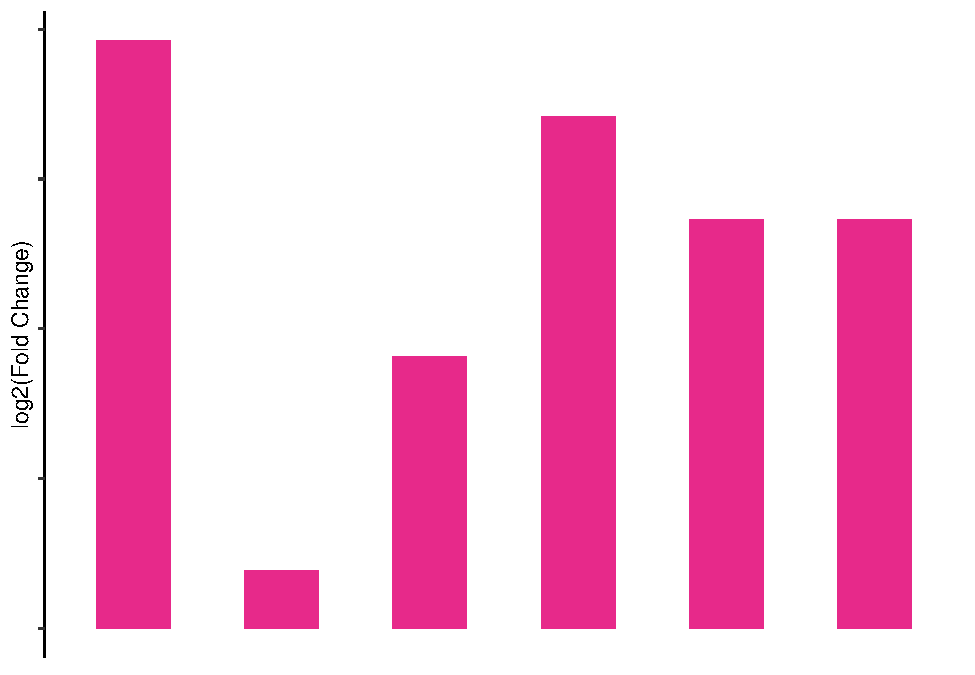
\includegraphics{ReadMe1_files/figure-latex/unnamed-chunk-17-2.pdf}

\begin{Shaded}
\begin{Highlighting}[]
\CommentTok{# Bottom plot}
\NormalTok{botAnn <-}\StringTok{ }\NormalTok{geneData }\OperatorTok
\StringTok{  }\KeywordTok{mutate}\NormalTok{(}\DataTypeTok{meth_f =} \KeywordTok{factor}\NormalTok{(gene, bottom)) }\OperatorTok
\StringTok{  }\KeywordTok{ggplot}\NormalTok{(}\DataTypeTok{mapping =} \KeywordTok{aes}\NormalTok{(}\DataTypeTok{x=}\NormalTok{gene,}\DataTypeTok{y=}\OperatorTok{-}\NormalTok{lfc)) }\OperatorTok{+}
\StringTok{  }\KeywordTok{geom_bar}\NormalTok{(}\DataTypeTok{fill =}\NormalTok{  RColorBrewer}\OperatorTok{::}\KeywordTok{brewer.pal}\NormalTok{(}\DecValTok{8}\NormalTok{, }\StringTok{"Dark2"}\NormalTok{)[}\KeywordTok{c}\NormalTok{(}\DecValTok{1}\OperatorTok{:}\DecValTok{5}\NormalTok{,}\DecValTok{7}\OperatorTok{:}\DecValTok{9}\NormalTok{)][}\DecValTok{2}\NormalTok{],}
           \DataTypeTok{stat =} \StringTok{"identity"}\NormalTok{,}
           \DataTypeTok{width =} \FloatTok{0.5}\NormalTok{) }\OperatorTok{+}
\StringTok{  }\KeywordTok{labs}\NormalTok{(}\DataTypeTok{x =} \OtherTok{NULL}\NormalTok{, }\DataTypeTok{y =} \StringTok{"Difference"}\NormalTok{) }\OperatorTok{+}
\StringTok{  }\NormalTok{theme_use2}
\NormalTok{botAnn}
\end{Highlighting}
\end{Shaded}

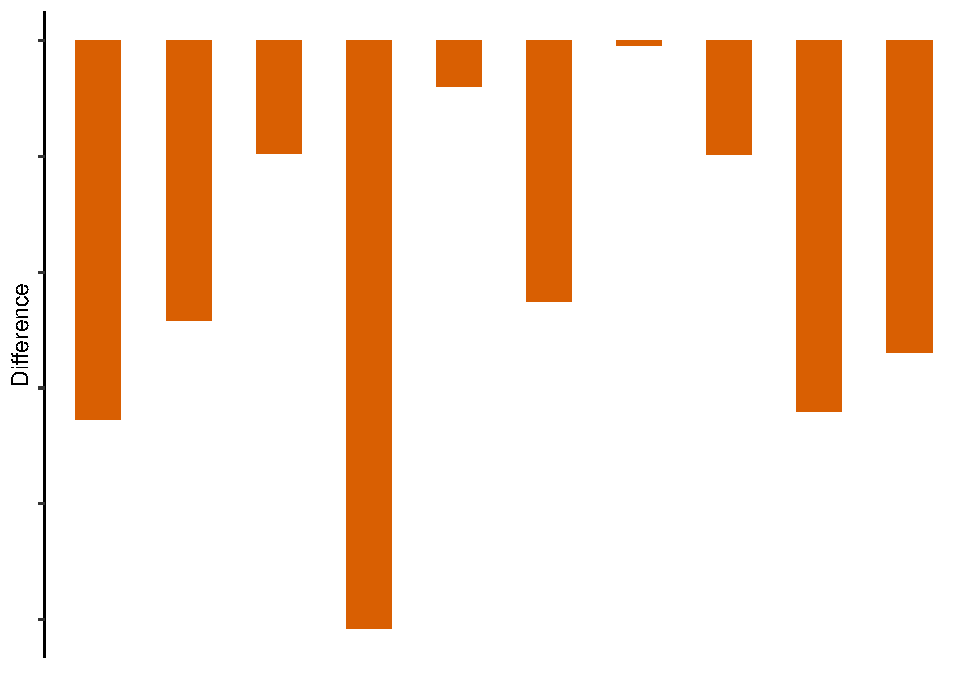
\includegraphics{ReadMe1_files/figure-latex/unnamed-chunk-17-3.pdf}

\begin{Shaded}
\begin{Highlighting}[]
\CommentTok{# right plot}
\NormalTok{rgtAnn <-}\StringTok{ }\NormalTok{methData }\OperatorTok
\StringTok{  }\KeywordTok{mutate}\NormalTok{(}\DataTypeTok{mir_f =} \KeywordTok{factor}\NormalTok{(meth, right)) }\OperatorTok
\StringTok{  }\KeywordTok{ggplot}\NormalTok{(}\DataTypeTok{mapping =} \KeywordTok{aes}\NormalTok{(}\DataTypeTok{x=}\NormalTok{meth,}\DataTypeTok{y=}\OperatorTok{-}\NormalTok{lfc)) }\OperatorTok{+}
\StringTok{  }\KeywordTok{geom_bar}\NormalTok{(}\DataTypeTok{fill =}\NormalTok{ RColorBrewer}\OperatorTok{::}\KeywordTok{brewer.pal}\NormalTok{(}\DecValTok{8}\NormalTok{, }\StringTok{"Dark2"}\NormalTok{)[}\KeywordTok{c}\NormalTok{(}\DecValTok{1}\OperatorTok{:}\DecValTok{5}\NormalTok{,}\DecValTok{7}\OperatorTok{:}\DecValTok{9}\NormalTok{)][}\DecValTok{3}\NormalTok{],}
           \DataTypeTok{stat =} \StringTok{"identity"}\NormalTok{, }
           \DataTypeTok{width =} \FloatTok{0.5}\NormalTok{) }\OperatorTok{+}
\StringTok{  }\KeywordTok{labs}\NormalTok{(}\DataTypeTok{x =} \OtherTok{NULL}\NormalTok{, }\DataTypeTok{y =} \StringTok{"log2(Fold Change)"}\NormalTok{) }\OperatorTok{+}
\StringTok{  }\NormalTok{theme_use2 }\OperatorTok{+}
\StringTok{  }\KeywordTok{coord_flip}\NormalTok{()}

\NormalTok{rgtAnn}
\end{Highlighting}
\end{Shaded}

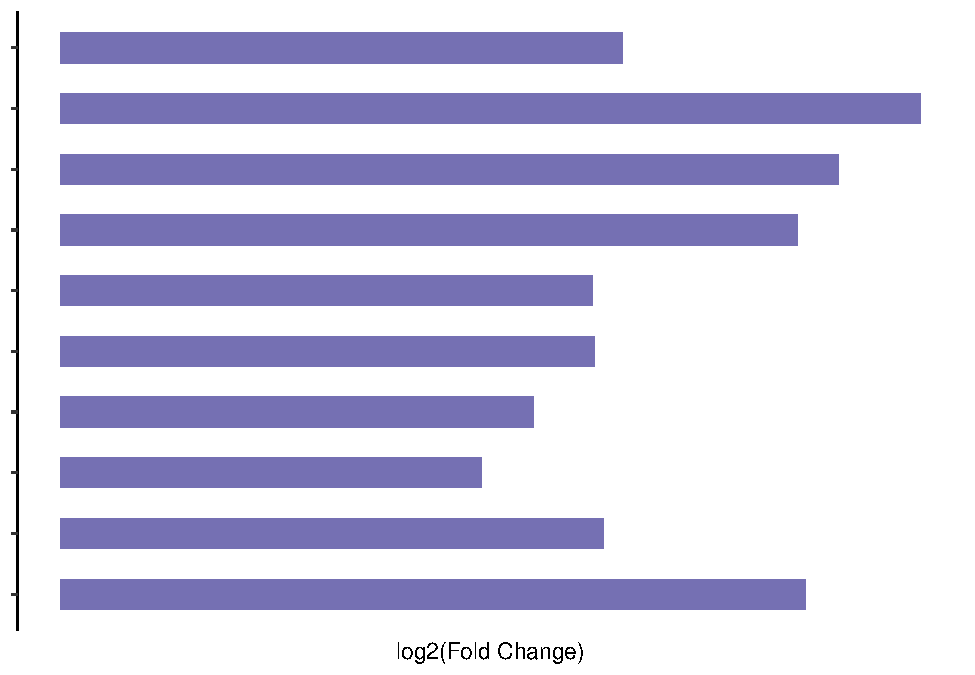
\includegraphics{ReadMe1_files/figure-latex/unnamed-chunk-17-4.pdf}

\begin{Shaded}
\begin{Highlighting}[]
\CommentTok{# left plot}
\NormalTok{mat =}\StringTok{ }\KeywordTok{matrix}\NormalTok{(}\KeywordTok{sample}\NormalTok{(}\DecValTok{1}\OperatorTok{:}\DecValTok{100}\NormalTok{, }\DecValTok{64}\NormalTok{, }\DataTypeTok{replace =}\NormalTok{ T), }\DataTypeTok{nrow =} \DecValTok{8}\NormalTok{)}
\KeywordTok{colnames}\NormalTok{(mat)=}\KeywordTok{as.character}\NormalTok{(cl}\OperatorTok{@}\NormalTok{cross}\OperatorTok{$}\NormalTok{Drug)}
\KeywordTok{ggplot}\NormalTok{(}\DataTypeTok{data =} \KeywordTok{melt}\NormalTok{(mat), }\KeywordTok{aes}\NormalTok{(X1, X2, }\DataTypeTok{fill =}\NormalTok{ value))}\OperatorTok{+}
\StringTok{     }\KeywordTok{geom_tile}\NormalTok{(}\DataTypeTok{color =} \StringTok{"white"}\NormalTok{)}\OperatorTok{+}\StringTok{ }
\StringTok{     }\KeywordTok{scale_fill_gradient2}\NormalTok{(}\DataTypeTok{low =} \StringTok{"blue"}\NormalTok{, }\DataTypeTok{high =} \StringTok{"darkgreen"}\NormalTok{, }\DataTypeTok{mid =} \StringTok{"white"}\NormalTok{,}\DataTypeTok{midpoint =} \DecValTok{0}\NormalTok{) }\OperatorTok{+}\StringTok{ }
\StringTok{     }\KeywordTok{xlab}\NormalTok{(}\StringTok{""}\NormalTok{)}\OperatorTok{+}\KeywordTok{ylab}\NormalTok{(}\StringTok{""}\NormalTok{)}\OperatorTok{+}\KeywordTok{theme_classic}\NormalTok{()}\OperatorTok{+}
\StringTok{     }\KeywordTok{theme}\NormalTok{(}\DataTypeTok{legend.position =} \StringTok{"right"}\NormalTok{,}
          \DataTypeTok{axis.line =} \KeywordTok{element_blank}\NormalTok{(),}
          \DataTypeTok{axis.ticks =} \KeywordTok{element_blank}\NormalTok{(),}
           \DataTypeTok{axis.text =} \KeywordTok{element_blank}\NormalTok{()) ->}\StringTok{ }\NormalTok{lftAnno}
\NormalTok{lftAnno}
\end{Highlighting}
\end{Shaded}

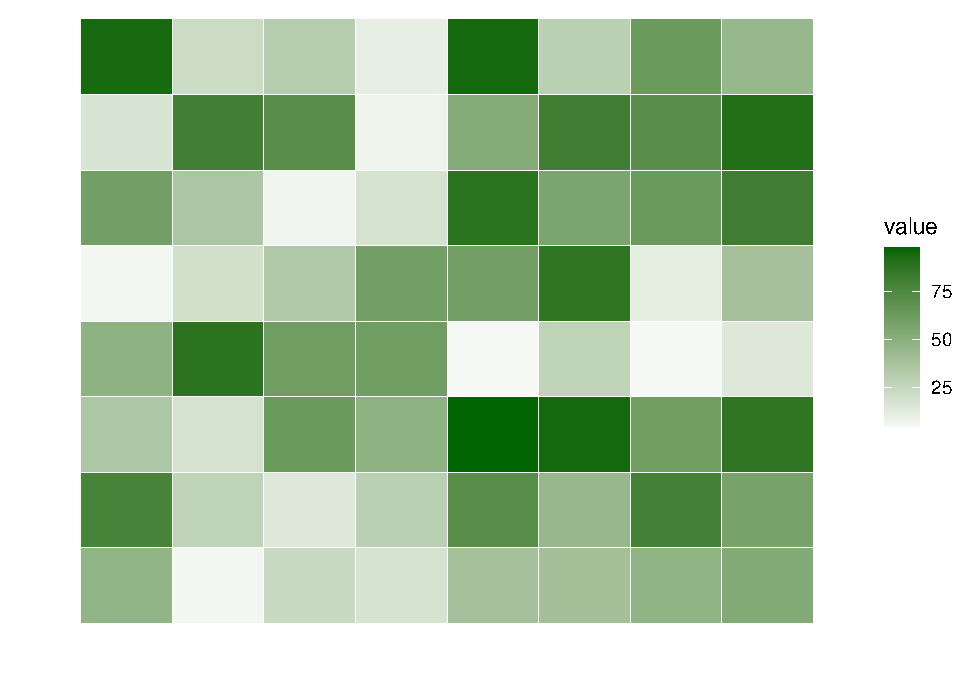
\includegraphics{ReadMe1_files/figure-latex/unnamed-chunk-17-5.pdf}

\begin{Shaded}
\begin{Highlighting}[]
\KeywordTok{cl_plot}\NormalTok{(cl,}
       \DataTypeTok{annotation=}\KeywordTok{cl_annotation}\NormalTok{(}\DataTypeTok{top =}\NormalTok{ topAnn,}\DataTypeTok{top.by =} \StringTok{"Mir"}\NormalTok{,}\DataTypeTok{top.height =} \FloatTok{0.5}\NormalTok{,}
                                \DataTypeTok{bottom =}\NormalTok{ botAnn,}\DataTypeTok{bottom.by =} \StringTok{"Gene"}\NormalTok{,}\DataTypeTok{bottom.height =} \FloatTok{0.5}\NormalTok{,}
                                \DataTypeTok{right =}\NormalTok{ rgtAnn,}\DataTypeTok{right.by =}\StringTok{"Meth"}\NormalTok{,}\DataTypeTok{right.width =} \FloatTok{0.5}\NormalTok{,}
                                \DataTypeTok{left =}\NormalTok{ lftAnno,}\DataTypeTok{left.by =} \StringTok{"Drug"}\NormalTok{ ,}\DataTypeTok{left.width =} \FloatTok{0.5}\NormalTok{),}
       \DataTypeTok{cross =} \KeywordTok{list}\NormalTok{( }\DataTypeTok{mapping =} \KeywordTok{aes}\NormalTok{(}\DataTypeTok{color =}\NormalTok{ type,}\DataTypeTok{size=}\NormalTok{degree,}\DataTypeTok{shape=}\NormalTok{type),}
       \DataTypeTok{scale =} \KeywordTok{list}\NormalTok{(}\DataTypeTok{color =} \KeywordTok{scale_color_manual}\NormalTok{(}\DataTypeTok{values =}\NormalTok{ RColorBrewer}\OperatorTok{::}\KeywordTok{brewer.pal}\NormalTok{(}\DecValTok{8}\NormalTok{, }\StringTok{"Dark2"}\NormalTok{)[}\KeywordTok{c}\NormalTok{(}\DecValTok{1}\OperatorTok{:}\DecValTok{5}\NormalTok{,}\DecValTok{7}\OperatorTok{:}\DecValTok{9}\NormalTok{)]),}
       \DataTypeTok{shape =} \KeywordTok{scale_shape_manual}\NormalTok{(}\DataTypeTok{values =} \DecValTok{15}\OperatorTok{:}\DecValTok{23}\NormalTok{),}
       \DataTypeTok{size  =} \KeywordTok{scale_size_continuous}\NormalTok{(}\DataTypeTok{range=}\KeywordTok{c}\NormalTok{(}\DecValTok{1}\NormalTok{,}\DecValTok{5}\NormalTok{)))),}
       \DataTypeTok{link  =} \KeywordTok{list}\NormalTok{(}\DataTypeTok{mapping =} \KeywordTok{aes}\NormalTok{(}\DataTypeTok{color =}\NormalTok{ type,}\DataTypeTok{linetype=}\NormalTok{type,}\DataTypeTok{size=}\NormalTok{cor),}
                    \DataTypeTok{scale =} \KeywordTok{list}\NormalTok{(}\DataTypeTok{color =} \KeywordTok{scale_color_manual}\NormalTok{(}\DataTypeTok{values =}\NormalTok{ RColorBrewer}\OperatorTok{::}\KeywordTok{brewer.pal}\NormalTok{(}\DecValTok{8}\NormalTok{, }\StringTok{"Set1"}\NormalTok{)[}\KeywordTok{c}\NormalTok{(}\DecValTok{1}\OperatorTok{:}\DecValTok{5}\NormalTok{,}\DecValTok{7}\OperatorTok{:}\DecValTok{9}\NormalTok{)]),}
                                \DataTypeTok{linetype=}\KeywordTok{scale_linetype_manual}\NormalTok{(}\DataTypeTok{values =} \KeywordTok{c}\NormalTok{(}\DecValTok{1}\OperatorTok{:}\DecValTok{4}\NormalTok{)),}
                                \DataTypeTok{size=}\KeywordTok{scale_size}\NormalTok{(}\DataTypeTok{range =} \KeywordTok{c}\NormalTok{(}\FloatTok{0.5}\NormalTok{,}\FloatTok{1.5}\NormalTok{)))),}
       \DataTypeTok{header=}\OtherTok{NA}\NormalTok{,}
       \DataTypeTok{label =} \KeywordTok{list}\NormalTok{(}\DataTypeTok{color=}\StringTok{"black"}
\NormalTok{                    ,}\DataTypeTok{angle=}\KeywordTok{c}\NormalTok{(}\KeywordTok{rep}\NormalTok{(}\DecValTok{0}\NormalTok{,}\DecValTok{8}\NormalTok{),}\KeywordTok{rep}\NormalTok{(}\DecValTok{90}\NormalTok{,}\DecValTok{10}\NormalTok{),}\KeywordTok{rep}\NormalTok{(}\DecValTok{0}\NormalTok{,}\DecValTok{10}\NormalTok{),}\KeywordTok{rep}\NormalTok{(}\DecValTok{90}\NormalTok{,}\DecValTok{6}\NormalTok{))}
\NormalTok{                    ,}\DataTypeTok{nudge_x=}\KeywordTok{c}\NormalTok{(}\KeywordTok{rep}\NormalTok{(}\OperatorTok{-}\DecValTok{2}\NormalTok{,}\DecValTok{8}\NormalTok{),}\KeywordTok{rep}\NormalTok{(}\DecValTok{0}\NormalTok{,}\DecValTok{10}\NormalTok{),}\KeywordTok{rep}\NormalTok{(}\DecValTok{2}\NormalTok{,}\DecValTok{10}\NormalTok{),}\KeywordTok{rep}\NormalTok{(}\DecValTok{0}\NormalTok{,}\DecValTok{6}\NormalTok{))}
\NormalTok{                    ,}\DataTypeTok{nudge_y=}\KeywordTok{c}\NormalTok{(}\KeywordTok{rep}\NormalTok{(}\DecValTok{0}\NormalTok{,}\DecValTok{8}\NormalTok{),}\KeywordTok{rep}\NormalTok{(}\OperatorTok{-}\DecValTok{2}\NormalTok{,}\DecValTok{10}\NormalTok{),}\KeywordTok{rep}\NormalTok{(}\DecValTok{0}\NormalTok{,}\DecValTok{10}\NormalTok{),}\KeywordTok{rep}\NormalTok{(}\DecValTok{2}\NormalTok{,}\DecValTok{6}\NormalTok{))),}
       \DataTypeTok{add   =}  \KeywordTok{theme}\NormalTok{(}\DataTypeTok{panel.background =} \KeywordTok{element_blank}\NormalTok{(),}\DataTypeTok{axis.title =} \KeywordTok{element_blank}\NormalTok{(),}
                      \DataTypeTok{panel.grid =} \KeywordTok{element_blank}\NormalTok{(),}
                      \DataTypeTok{axis.ticks =} \KeywordTok{element_blank}\NormalTok{(),}
                      \DataTypeTok{axis.text =} \KeywordTok{element_blank}\NormalTok{()))}
\end{Highlighting}
\end{Shaded}

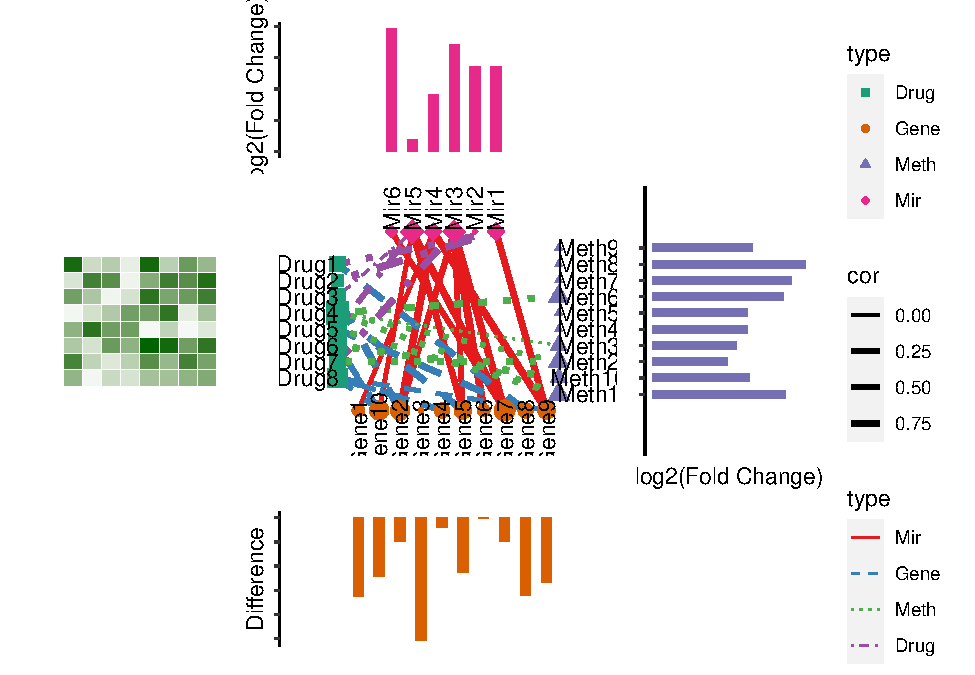
\includegraphics{ReadMe1_files/figure-latex/unnamed-chunk-17-6.pdf}

\end{document}
